\part{Experimental control}
\label{part:experiment}

\chapter{Experimental Testbed and Experiment Engines}%
\label{chapter:experiment:testbed}

    \section{State of the art}%
    \label{sec:state_of_the_art}

        \subsection{Grid'5000}%
        \label{sub:grid_5000}

            Nearly all the experiments presented in this document have been carried on the Grid'5000~\cite{grid5000}
            testbed.  Quoting its official website\footnote{\url{https://www.grid5000.fr/}}: \blockquote{Grid'5000 is a
            large-scale and flexible testbed for experiment-driven research in all areas of computer science, with a
            focus on parallel and distributed computing including Cloud, HPC and Big Data and AI.} It provides dozen of
            clusters, each one having between 2 and 124 homogeneous compute nodes. There is a high diversity of hardware,
            including several generations of Intel processors available, AMD and ARM processors, GPU, persistent memory
            (PMEM) as well as high-performance networks such as Infiniband or Omni-path. Another important feature is the
            ability for the experimenter to get full control on the nodes, as it is possible to deploy a new operating
            system and therefore to gain superuser access.

        \subsection{Experiment engines}%
        \label{sub:experiment_engines}

            While it is possible to run a complete experiment on a testbed like Grid'5000 by manually issuing commands
            in an interactive shell, it is not advisable as it quickly becomes extremly tedious and error-prone.
            Automating the experiment is a necessary condition to have reproducible results. A first step toward this
            goal is to write some ad-hoc script. However, two independent experiments might still share a lot of steps
            that could be refactored in a common layer, \eg OS deployment, package installation, or even more advanced
            features like node instrumentation or environment logging.

            For these reasons, it is a common practice to use an experiment engine. Buchert~\etal describe the features
            of eight different softwares~\cite{buchert:hal-01087519}. To the best of our knowledge, only three offer a
            native support for Grid'5000, namely Expo, XPFlow and Execo. Unfortunately, Expo and XPFlow are now longer
            maintained, the last commit in their respective repositories was done on November 2014 and September 2015
            For these reasons, the experiment engine Execo~\cite{Imbert_2013} is often recommended to Grid'5000
            newcomers.

            Experiments with Execo are described as a Python script. We believe this is one of its best qualities, as it
            offers a lot of freedom and flexibility to the experimenter, comparatively to other experiment engines that
            use custom domain specific languages (DSL). Yet, we made the choice to not use it. The main reason is that a
            typical Execo experiment uses a lot of low-level constructs that are really unpleasant and unintuitive to
            write and read. Section~\ref{sub:comparison_with_execo} will present some comparisons. Furthermore, Execo
            lacks a lot of important features, like node instrumentation and metadata collection, \ie we would still
            have needed to implement a lot functionnalities on top of Execo.

    \section{Yet another experiment engine: \texttt{peanut}}%
    \label{sec:peanut}
        %% TODO
        %% Différents moyens mis en oeuvre pour faciliter la reproductibilité (au sens
        %% large) :
        %% - Description structurée et lisible d'une expérience, relativement haut niveau
        %%   -> on comprend facilement ce qu'il se passe, on peut reproduire l'expérience
        %%   sans utiliser peanut.
        %% - Une fois l'expérience écrite, 100% automatisé, lancée avec juste une ligne de
        %%   commande.
        %% - Collecte d'information : commandes exécutées et leur std{out,err},
        %%   informations système, timestamps, monitoring.
        %% - Attention aux excès, pas forcément pertinent de collecter 10GB
        %%   d'info par expérience, voir même contre-productif si ça incite à ne
        %%   pas refaire les XP. Parler des problèmes découverts sur G5K (ref. au
        %%   dernier chapitre) ?
        %% - Future work: NIX & GUIX.
        %% - L'utilisateur garde le contrôle sur le plan d'expérience, grâce à des fichiers
        %%   d'expériences (peanut n'est pas chargé de randomiser l'xp). Ref à la prochaine
        %%   section.
        \subsection{Key features}%
        \label{sub:key_features}
            We implemented our own experiment engine, named \texttt{peanut}. It comes as a Python library that
            experimenters can use to write their own experiments, also as a Python script.

            A new experiment can be defined by inheriting from the class \texttt{peanut.Job}. Three methods can be
            overriden, \texttt{setup}, \texttt{run\_exp} and \texttt{teardown}.

            Once the experiment is written, it can be launched in a single command line. The following steps will
            happen.
            \begin{itemize}
                \item Implicitely, submit a job with the given characteristics (\eg cluster, number of nodes, walltime,
                    etc), then deploy the given OS image.
                \item Implicitely (but optionnaly) enable or disable some performance functionnalities like
                    hyperthreading, turboboost, C-states.
                \item Implicitely (but optionnaly) instrument the nodes to collect at a regular interval some system
                    metrics (\eg core frequencies and temperatures, CPU power consumption, network traffic, memory
                    consumption).
                \item Implicitely (but optionnaly) run the \texttt{stress} command on all the nodes to warm them up.
                \item Run the methods \texttt{setup}, \texttt{run\_exp} and \texttt{teardown} in that order.
                \item Produce a \texttt{zip} archive containing relevant results and metadata. The experimenter can
                    explicitely add any file to the archive. In addition, the following content is also implicitely
                    archived:
                    \begin{itemize}
                        \item Metrics collected with the aforementioned instrumentation.
                        \item Human-readable log of the commands issued during the experiment.
                        \item Machine-parsable log of the commands (in JSON format) with their timestamps and output
                            (both \texttt{stdin} and \texttt{stderr}).
                        \item Machine-parsable file (in Yaml format) containing relevant information like
                            the exact versions used for \texttt{peanut}, \texttt{gcc}, \texttt{MPI} and the Linux
                            kernel, the command line that was used to launch this experiment, the cluster and the list
                            of nodes, start and end timestamps for each of the three main methods, the list of the git
                            repositories cloned during this experiment with their remote URL and the git hash of the
                            checkout.
                        \item For each node, the content of the file \texttt{/proc/cpuinfo} as well as the output of the
                            commands \texttt{env}, \texttt{lstopo}, \texttt{lspci}, \texttt{dmidecode},
                            \texttt{lsmod}, \texttt{dmesg}.
                    \end{itemize}
            \end{itemize}
            In addition, the experiment can be executed interactively in a Python terminal. All the implicit
            functionnalities described previously can also be explicitely called (\eg there are methods
            \texttt{disable\_hyperthreading}, \texttt{start\_monitoring} and \texttt{perform\_stress}).

            An experiment can be parametrized by two means:
            \begin{itemize}
                \item An install file. This is a Yaml file that can be used to describe how the setup phase should be
                    done. Typically, it can contain the desired version for different softwares like OpenBLAS or
                    OpenMPI, but also the duration of the warmup or the frequency of the monitoring.
                \item An experiment file. These can be of any kind. A typical use case is to provide a CSV file where
                    each line is a particular piece of the experiment (\eg an individual call to \dgemm and the
                    columns represent the parameters for these experiments (\eg the sizes \texttt{M}, \texttt{N} and
                    \texttt{K} used by \dgemm).
            \end{itemize}

        \subsection{Comparison with Execo}%
        \label{sub:comparison_with_execo}

            In this section, we use a small example to illustrate some differences between \texttt{peanut} and
            \texttt{execo}. The goal is to write an experiment that will take several nodes on a given Grid'5000
            cluster, compile the \texttt{CRoaring} library\footnote{\url{https://github.com/RoaringBitmap/CRoaring}} and
            run one of its benchmarks.

            \lstdefinestyle{custom_lst_style}{
             %   language=Matlab,
                numbers=left,
                stepnumber=1,
                numbersep=10pt,
                tabsize=4,
                showspaces=false,
                showstringspaces=false
            }
            \lstset{basicstyle=\scriptsize, style=custom_lst_style}

            First, Listing~\ref{lst:engine:execo} shows such an experiment using Execo. Run with: \verb#python script.py#\\

            \lstinputlisting[language={Python},label={lst:engine:execo},
                caption={Small experiment example Execo}]{
                img/experiment/engine/mweExeco.py
            }

            This script, albeit fairly small, is already difficult to read in some places. For instance, lines 11-12,
            one has to write a complex query as a string as follows:

            \verb#OarSubmission("{cluster in ('dahu')}/nodes=2,walltime=00:20:00")#

            It would be much more pleasant to write it as follows:

            \verb#OarSubmission(cluster="dahu", nodes=2, walltime="00:20:00")#

            Now, Listing~\ref{lst:engine:peanut_class} demonstrates how the same experiment can be rewritten using Peanut
            in a much more concise and readable way.

            Run with: \verb#peanut script.py run tocornebize --deploy debian9-x64-base \#\\
            \verb#    --cluster dahu --nbnodes 2 --walltime 00:20:00#

            \lstinputlisting[language=Python,label={lst:engine:peanut_class},
                caption={Small experiment example using Peanut}]{
                img/experiment/engine/mwePeanut.py
            }

            The script is not only twice shorter, it is also much more elegant. Furthermore, it accomplishes much more
            than Listing~\ref{lst:engine:execo}, as it produces a peanut archive with all the metadata related to the
            experiment.

\chapter{Randomizing matters!}%
\label{chapter:experiment:randomizing}
    %% TODO
    %% Calibration experiments: randomisation. pour quoi faire ?
    %% 1. éviter les biais (randomisation de l'espace de paramètres)
    %%    - certaines valeurs peuvent être particulières et on peut vouloir
    %%      au contraire biaiser vers ces valeurs
    %% 2. éviter les perturbations transientes
    %%    - montée en charge vs. régime stationnaire
    %%
    %% Plusieurs exemples à citer (ref aux présentations qu'on aurrait dû
    %% faire à XUG@Rennes et à JLESC@Bonnes).
    Suppose some researcher wants to evaluate the memory bandwidth of their laptop. A first way to answer this question
    could be to write a small program that allocates a buffer, then write some data on this buffer with the
    \texttt{memset} function while measuring the duration of this operation. The problem is that the time taken to make
    this memory write may not be representative, the following writes would very probably have different durations due
    to cache effects.  Therefore, it would be better to make several measures that should then be carefuly analyzed
    (maybe simply taking the average, or perhaps there are some \emph{outliers} that should be removed). However, by
    doing so we only measure the performance of a write for a given size. The effective bandwidth could be very
    different with a smaller or a larger buffer. The natural solution here is to repeat these sequences of measures for
    several sizes.

    A general advice shared by experimental scientists in such situations is to randomize the experiments. In general,
    this randomization should happen for:
    \begin{itemize}
        \item The parameter space (in this example, the set of sizes that are evaluated). The goal is to avoid bias, for
            instance sizes that are a power of two may lead to a different performance. Note that in some occasions, as
            this chapter will illustrate, it is desirable to bias the experiment towards some particular values.
        \item The experiment order (in this example, the order of the sizes). The rational here is to avoid temporal
            perturbations. In particular, there are often at least two phases, a load build up which converges toward a
            steady state. There can also be changes that happen once the steady state is reached, \eg caused by some
            external source. By randomizing the order of the experiments, it becomes much easier to recognize an
            eventual temporal perturbation simply by plotting the data.
    \end{itemize}

    In this chapter, we will discuss several lessons learned for conducting faithful experiments, most of the time the
    hard way.

    \section{Experimental setup}%
    \label{sec:experimental_setup}

        All the experiments presented in this chapter share a common setup. They have been repeated on several nodes and
        follow the same steps:
        \begin{enumerate}
            \item Deploy and install a fresh OS on the node.
            \item Run the \texttt{stress} command for 10 minutes to warm the node.
            \item Start a background process\footnote{\url{https://github.com/Ezibenroc/ratatouille}} to monitor the
                core frequencies and temperature every second.
            \item On each core, run a custom
                code\footnote{\url{https://github.com/Ezibenroc/platform-calibration/src/calibration}}
                to measure the durations of a given operation (either \dgemm or several MPI functions, depending
                on the experiment).
        \end{enumerate}

        Unless specified otherwise, we used nodes from the Dahu cluster from
        Grid'5000\footnote{\url{https://www.grid5000.fr/w/Grenoble:Hardware}}. Each of these nodes has two Intel Xeon
        Gold 6130 CPU, which are 16 core CPU from the Skylake generation. They have a base frequency of
        \NSI{2.1}{\giga\hertz} and a turbo frequency of up to \NSI{3.7}{\giga\hertz}, but their turbo frequency is
        limited to \NSI{2.4}{\giga\hertz} when their 16 cores are active and in AVX2
        mode\footnote{\url{https://en.wikichip.org/wiki/intel/xeon\_gold/6130}}. We have used
        OpenBLAS\footnote{\url{https://github.com/xianyi/OpenBLAS}} version~0.3.1 and
        OpenMPI\footnote{\url{https://github.com/open-mpi/ompi}} version~2.0.2 compiled with GCC version~6.3.0 on a
        Debian~9 installation with kernel version~4.9.0.

    \section{Defining the parameter space}%
    \label{sec:parameter_space}

        Two families of experiments are discussed in this chapter: (1) MPI operations such as calls to
        \recv or \send, their duration is proportional to \(S\), the size of the buffer that is
        being communicated, and (2) calls to the \dgemm function, whose duration is proportional to the product
        of the sizes \(MNK\) but also depends on individual interactions of those sizes.

        An experiment consists in a sequence of calls to the function of interest, with various sizes as parameters. The
        goal of this section is to discuss how and why the parameters of these sequences are generated.

        \subsection{MPI communications}%

            If we assume that the duration of a communication is linear in the amount of data being sent, the easiest
            way to sample the data is to only measure two sizes, one very small buffer (\eg \NSI{1}{\byte}) and one very
            large buffer (\eg \NSI{1}{\giga\byte}). To avoid any bias, we could even try several small and large
            buffers with slight differences in their respective sizes. However, we saw in Part~\ref{part:prediction}
            that this linearity assumption does not hold, their are large discontinuities. We therefore need to also
            sample sizes between the two extreme values to (1) make sure that all the breakpoints are visible in our
            dataset and (2) perform one linear regression in each linear zone.

            Given this requirement, the natural sampling method would be a uniform sampling, taking
            \(S\sim\unif{1}{10^9}\). However, in our experiments, we found out that the breakpoints are not uniformly
            spread, but rather exponentially. For instance, the \send on the dahu cluster has four
            breakpoints: \NSI{8.14}{\kilo\byte}, \NSI{34.0}{\kilo\byte}, \NSI{63.8}{\kilo\byte} and
            \NSI{285}{\mega\byte}. If the sizes of the experiment were uniformly sampled, we would very probably miss
            the smaller breakpoints: by sampling uniformly and indepently 1000 numbers in the interval \([1, 10^9]\),
            the probability to have at least one number smaller or equal to \(10^5\) is a bit less than
            \NSI{10}{\percent}. The reason for these exponentialy spread breakpoints likely comes from the hardware.
            Typically, each layer of the memory hierarchy is one order of magnitude larger than the previous layer. For
            instance, each core of a dahu node has \NSI{32}{\kibi\byte} L1 instruction and data caches and one
            \NSI{1}{\mebi\byte} L2 cache. Then, the 16 cores of a same CPU share a \NSI{22}{\mebi\byte} L3 cache and
            a \NSI{93}{\gibi\byte} memory.

            For these reasons, we made the choice to sample the sizes exponentially in the considered interval. More
            precisely, each size $S$ is sampled as: \[S\sim10^{\unif{0}{9}}\]

        \subsection{Function \dgemm}%
        \label{sub:parameter_space:dgemm}

            The situation is different with the \dgemm function. We did not observe any breakpoint in the performance
            plots as for the MPI communications. Hence, we did not have any reason to use an exponential sampling. A
            first solution would therefore consist in taking \(M=N=K\) and sampling the product \(MNK\) uniformly in
            some interval.  This could be sufficient for a simple linear regression with only one parameter, but as
            discussed in Part~\ref{part:prediction} we need several coefficients of the polynomial. For this reason, we
            have to cover a larger zone of the parameter space.

            Two options have been considered. Suppose we would like the three sizes \(M,N,K\) to be smaller or equal to
            some constant \(\Sigma\) and their product \(MNK\) to be smaller or equal to some other constant \(\Pi\).
            \begin{description}
                \item[Independent sizes] Each of the three sizes \(M\), \(N\) and \(K\) is sampled independently and
                    uniformly in the desired interval:
                    \begin{enumerate}
                        \item \(M \sim \unif{1}{\Sigma}\) and \(N \sim \unif{1}{\Sigma}\) and
                            \(K \sim \unif{1}{\Sigma}\)
                        \item Repeat until \(MNK \leq \Pi\)
                        \item Return \((M,N,K)\)
                    \end{enumerate}
                    This is the easiest method to implement. With this approach, the product
                    \(MNK\) is not uniform, it is heavily skewed towards the small values. Additionaly, we use rejection
                    sampling to make sure that the product of the sizes does not get too large.
                \item[Uniform product] We start by sampling the size product \(P\) uniformly in the desired interval,
                    then the sizes \(M\), \(N\) and \(K\) are sampled randomly to get (approximately) the correct
                    product:
                    \begin{enumerate}
                        \item \(P \sim \unif{1}{\Pi}\)
                        \item \(A \sim \unif{1}{\sqrt[3]{P}}\)
                        \item \(B \sim \unif{1}{\sqrt{\frac{P}{A}}}\)
                        \item \(C = \frac{P}{AB}\)
                        \item Repeat steps 2 to 4 until \(A \leq \Sigma\) and \(B \leq \Sigma\) and \(C \leq \Sigma\)
                        \item Return the six possible permutations: \((M,N,K) = (A,B,C), (C,A,B), \dots\)
                    \end{enumerate}
                    The goal of returning all the permutations of the sizes is to avoid any bias in the sampling
                    procedure, since they are not generated independently from each other. We also use rejection
                    sampling to make sure that one of the sizes does not get too large.
            \end{description}

            These two generation methods are illustrated in Figure~\ref{fig:parameter_space}. A list of \Num{100000}
            size tuples was sampled with each approach.

            \begin{figure}[htpb]
                \centering
                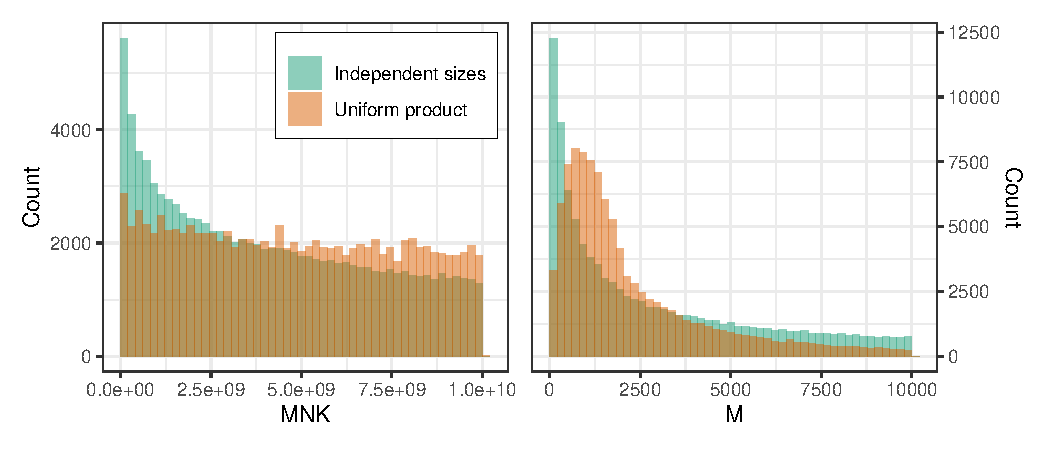
\includegraphics[width=\linewidth]{img/experiment/parameter_space/distribution.pdf}
                \caption{Distribution of the product \(MNK\) and the size \(M\) with the two generation methods. The
                maximal product is set to \(10^{10}\) and the maximal size to \Num{10000}.}%
                \label{fig:parameter_space}
            \end{figure}

            The left plot shows that as expected, the product \(MNK\) appears to have a large left-skew with the first
            approach and to be uniformly distributed with the second approach. The right plot is more surprising, since
            the parameter \(M\) is not uniformly distributed with the first approach. The reason is the rejection
            sampling, large values for \(M\) are more likely to give a product \(MNK\) above the specified limit and
            thus to be rejected.

            Since the product \(MNK\) is the most significant factor for the duration of \dgemm, it is more natural to
            use a uniform distribution for this term, we therefore made the choice to use the second approach for
            generating experiment files for the \dgemm experiments, with two minor modifications:
            \begin{itemize}
                \item Instead of sampling the product uniformly with \(MNK\sim\unif{1}{S}\), we made the choice to use a
                    slightly more deterministic approach. We first compute $\gamma$ different values that are uniformly
                    but deterministically spread in the given interval, \ie we compute the set
                    \(\left\{S, S-\frac{S}{\gamma},S-2\frac{S}{\gamma}, \dots\right\}\)
                    (typically, \(\gamma=30\)). Then we add a random noise independently to each of these sizes. The
                    goal is to ensure a similar (yet still random) distribution of the products \(MNK\) each time we
                    generate a new experiment file. This approach is similar to latin hypercube sampling (LHS).
                \item In addition of the size tuples randomly generated, we systematically add a few tuples to the list,
                    like \((1,1,1)\) or \((2048,2048,2048)\). The goal is to ensure that we have a few identical calls to
                    \dgemm in every experiment, in case we want a fine comparison.
            \end{itemize}

    \section{Randomizing the order}%
    \label{sec:randomizing_order}
        The network model in SMPI needs to be instanciated with a careful calibration of the MPI communication
        performance, as presented in \cite{smpi}. This was done with a MPI program created by the Simgrid team that
        performed a sequence of measures with two hosts. Several kind of measures were implemented: the \emph{recv}
        (a call to \recv with waiting to avoid late senders), the \emph{isend} (a call to
        \texttt{MPI\_Isend}), the \emph{pingpong} (a call to \send followed by a call to \recv
        to get the round-trip time) as well as several more minor MPI primitives.

        \begin{algorithm}[H]
            read the sequence of sizes \(S_1\), typically \(|S_1| \approx 1000\)\;
            \(S_2 := \underbrace{S_1\cdot S_1\cdot\dots\cdot S_1}_{N\text{ concatenations, typically } N\approx 50}\)\;
            \For{each kind of measure (recv, isend, pingpong, etc.)}{
                \For{\(s \in S_2\)}{
                    perform the measure $K\approx10$ times and output each individual duration
                }
            }
        \end{algorithm}

        Although the sequence of sizes \(S_1\) is a random sequence, there are still two obvious biases in this
        experiment.  First, the final sequence \(S_2\) is a concatenation of several instances of \(S_1\), so the same
        (random) order will be used in these \(N\) runs. Then, the different kind of measures are performed one after
        the other.

        In a first step towards a better methodology, we started by shuffling entirely the sequence \(S_2\) after the
        concatenation. The observed durations for function \recv with both methods are presented in
        Figure~\ref{fig:randomizing_order:raw_data}. There is no obvious difference here, in both cases the duration is
        piecewise linear in the message size and several modes are present for the small and medium messages.

        \begin{figure}[htpb]
            \centering
            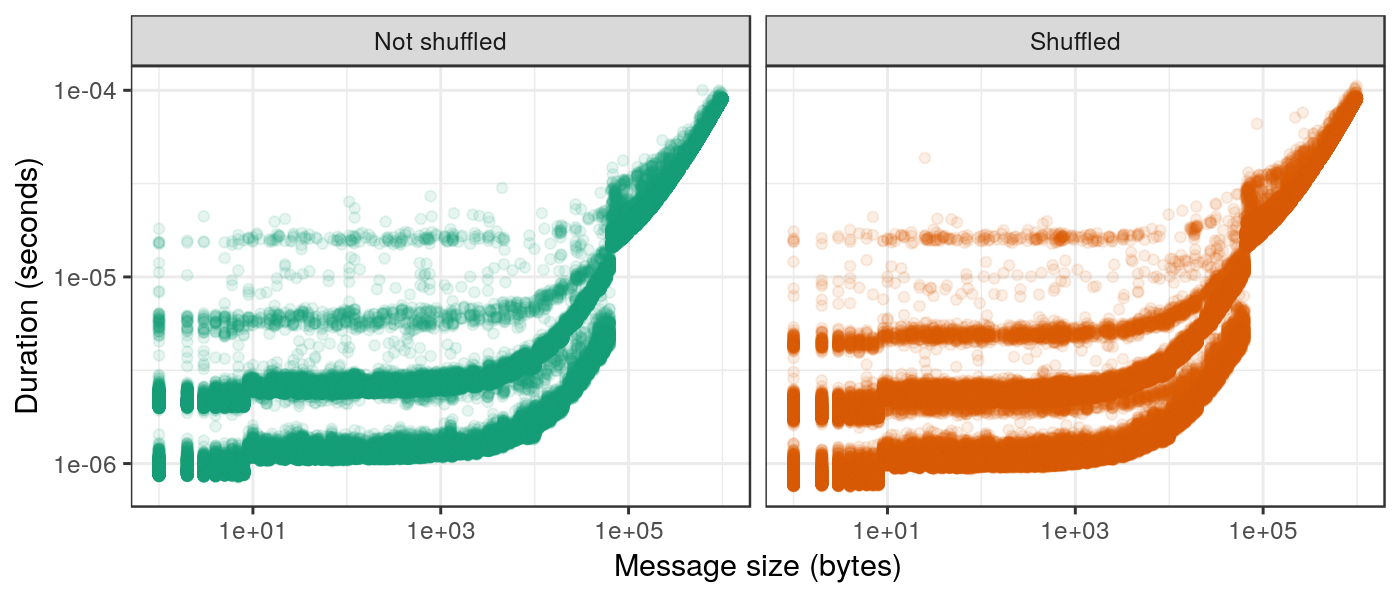
\includegraphics[width=\linewidth]{img/experiment/randomizing_order/raw_data.png}
            \caption{The duration of \recv is piecewise linear, with several modes for small messages.}%
            \label{fig:randomizing_order:raw_data}
        \end{figure}

        To compute a network model for SMPI, we need to perform a (segmented) linear regression on this data. One
        assumption for the simple least-square regression is that the noise should be normaly distributed, which is
        clearly not the case with our dataset, the noise is multi-modal. One simple solution for this is to compute the
        average duration for each message size, which all have a large number of measures (500 in this figure). With the
        central limit theorem, assuming that the measures for similar message sizes are independent and identically
        distributed, their sample average is normaly distributed. This means that by averaging the data, we should get a
        normal noise which would allow us to compute a linear regression.

        \begin{figure}[htpb]
            \centering
            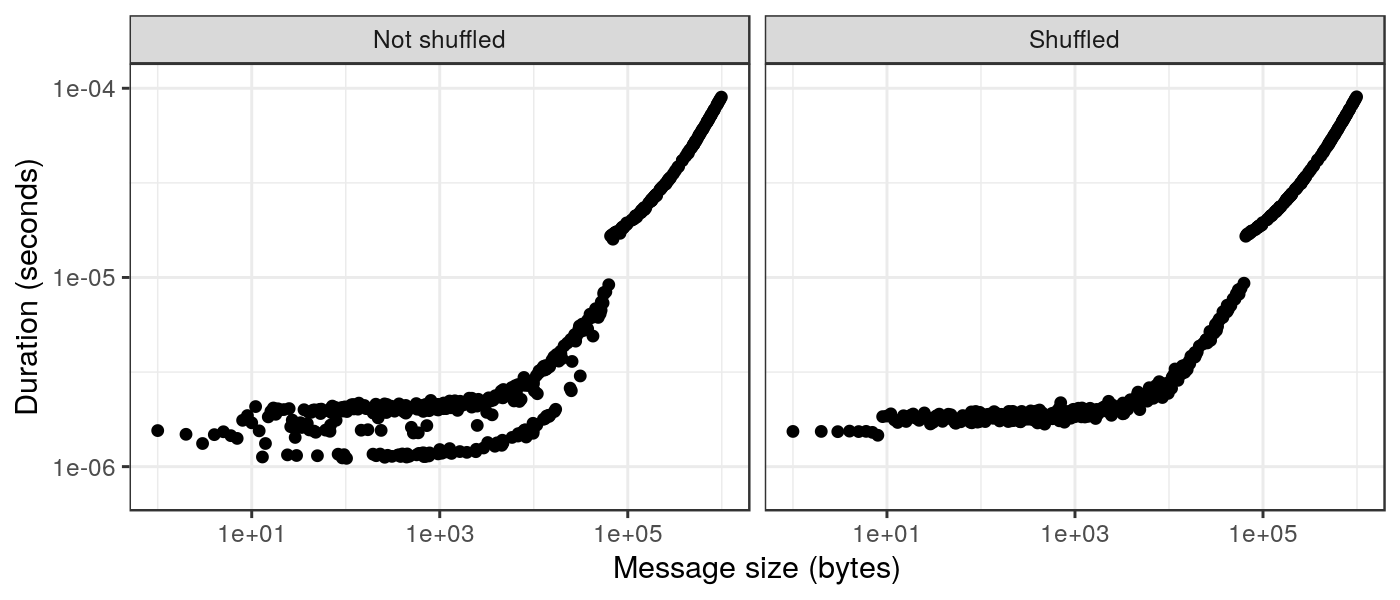
\includegraphics[width=\linewidth]{img/experiment/randomizing_order/aggregated_data.png}
            \caption{The average durations of \recv in the non-shuffled case still show several modes,
            which should not happen according to the central limit theorem.}%
            \label{fig:randomizing_order:avg_data}
        \end{figure}

        The aggregated data is presented in Figure~\ref{fig:randomizing_order:avg_data}. With the shuffled experiment
        (right plot), the average durations have a single-mode, as expected. However, in the non-shuffled case (left
        plot), at least two modes are clearly present. This contradicts the conclusion of the central limit theorem,
        thereby proving that its hypotheses do not hold for this experiment. This is confirmed by
        Figure~\ref{fig:randomizing_order:distribution}, where we zoomed on a few distinct message sizes between
        \NSI{700}{\byte} and \NSI{800}{\byte}. Each point is the duration of an individual call to \recv,
        the crosses represent the average durations. In the shuffled experiment, on the right, the duration
        distributions are similar for all message sizes, with two modes clearly identifiable and the average in between.
        In the non-shuffled case, on the left, the durations of three message sizes are different, namely
        \NSI{703}{\byte}, \NSI{767}{\byte} and \NSI{779}{\byte}. For these three calls, the distributions have only one
        mode, so their average durations are significantly shifted. The assumption of identical distribution for these
        different message sizes is clearly not satisfied here.

        \begin{figure}[htpb]
            \centering
            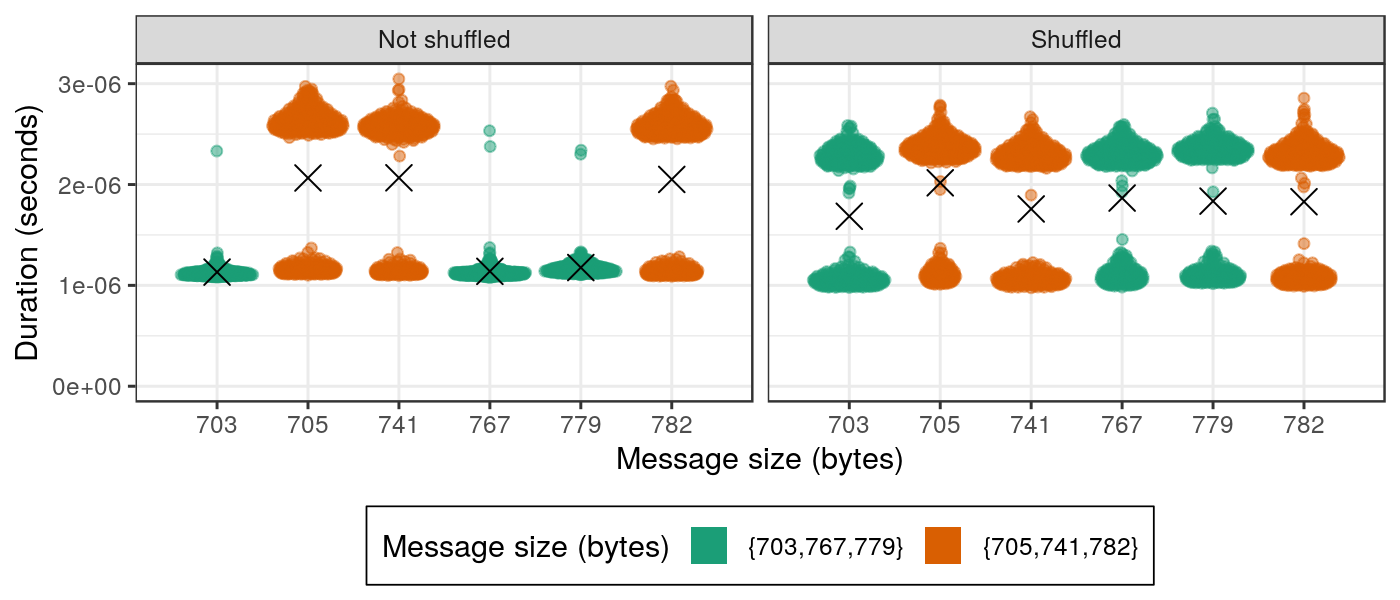
\includegraphics[width=\linewidth]{img/experiment/randomizing_order/distribution.png}
            \caption{Distribution of the \recv durations for six different message sizes between \NSI{700}{\byte} and
            \NSI{800}{\byte}.  The durations are not identically distributed in the non-shuffled case.  Durations
            truncated to \NSI{4}{\micro\second} for a better readability.}%
            \label{fig:randomizing_order:distribution}
        \end{figure}

        Since shuffling correctly the experiments prevents the occurence of this issue, a possible reason could be that
        the individual calls to \recv are not truly independent. The sequence before the calls for the sizes like
        \NSI{703}{\byte}, \NSI{767}{\byte} or \NSI{779}{\byte} would lead to particularly good conditions and thus an
        excellent performance, which does not systematically happen in the shuffled case because of the proper
        randomization. However, we could not identify anything suspect regarding the message sizes of the calls made
        just before these high-performance calls. Some of them had messages of a few bytes, some others had messages of
        several hundreds kilobytes.

        In Figure~\ref{fig:randomizing_order:evolution}, we present the temporal evolution of the durations for the
        calls to \recv made with the sizes presented in Figure~\ref{fig:randomizing_order:distribution}. In the
        non-shuffled case, we can identify a temporal pattern. During the first 20 seconds of the experiment, the
        calls with sizes \NSI{705}{\byte}, \NSI{741}{\byte} and \NSI{782}{\byte} (in green) have durations above
        \NSI{2}{\micro\second} for a large fraction of them, only a small part have durations below
        \NSI{1.5}{\micro\second}. After the 20 second timestamp, this suddenly changes, there are at least two time
        windows where all these calls have a low duration. Even outside these time windows, a much larger fraction of
        these calls have low durations. This temporal pattern is not visible in the other cases.

        \begin{figure}[htpb]
            \centering
            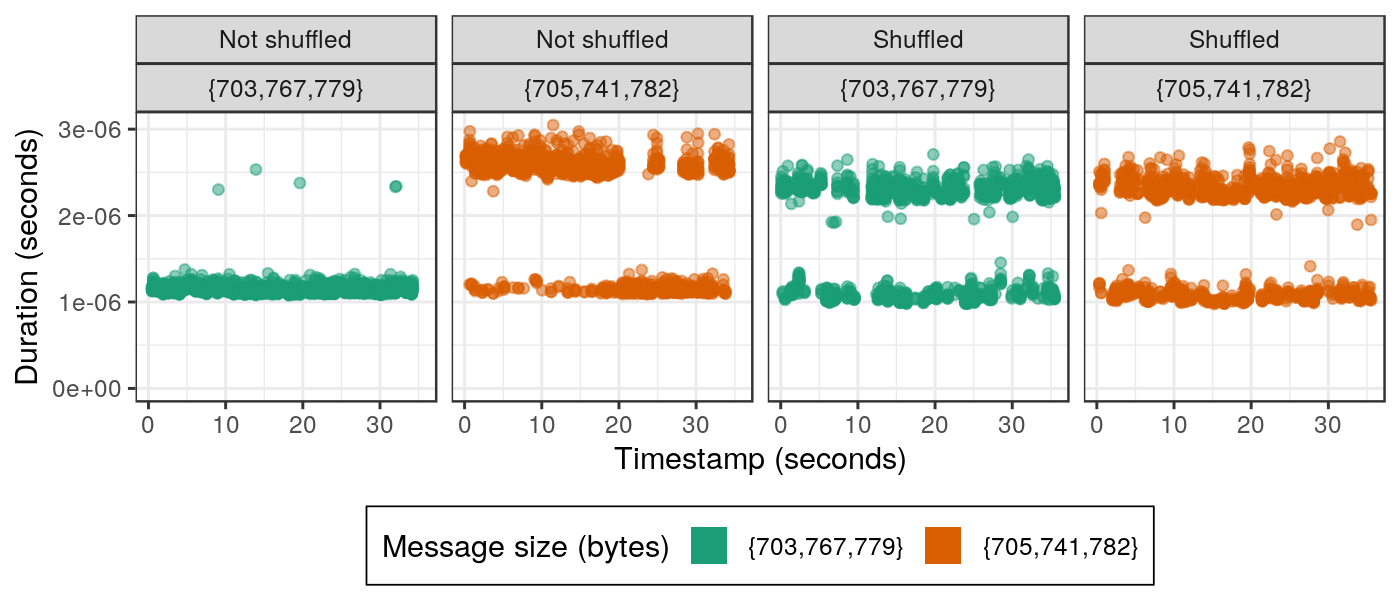
\includegraphics[width=\linewidth]{img/experiment/randomizing_order/evolution.png}
            \caption{Temporal evolution of the \recv durations for six different message sizes between \NSI{700}{\byte}
            and \NSI{800}{\byte}. A temporal pattern can be observed. Durations truncated to \NSI{4}{\micro\second} for
            a better readability.}%
            \label{fig:randomizing_order:evolution}
        \end{figure}

        Another view of the non-shuffled experiment is presented in Figure~\ref{fig:randomizing_order:evolution_rug}.
        Now all the calls with a size lower than \NSI{1}{\kilo\byte} are shown, but only a small fraction of the whole
        experiment is displayed. The calls to \recv can be divided into two groups depending on their durations, lower
        (in green) or greater (in orange) than \NSI{1.7}{\micro\second}. The rug plot on the top of the figure
        highlights the position in time of each of these \recv calls. Although there are slow and fast calls uniformly
        distributed during this time window, there appears to be some clusters where nearly all the calls are of the
        same kind.

        \begin{figure}[htpb]
            \centering
            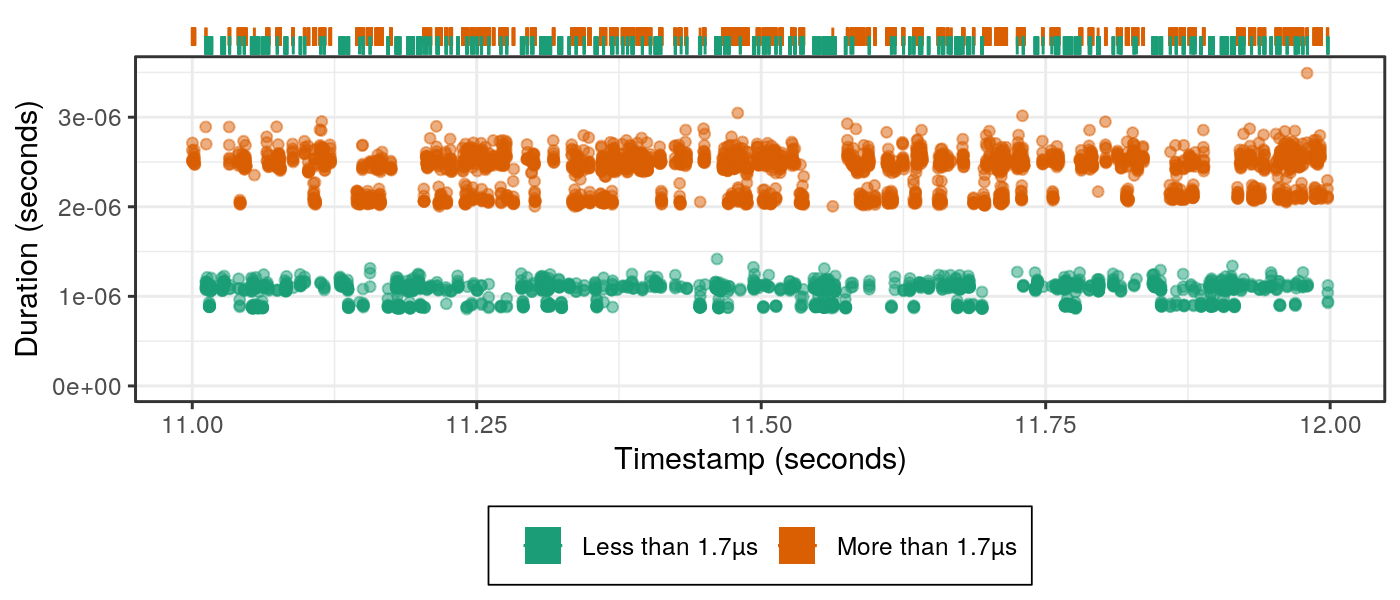
\includegraphics[width=\linewidth]{img/experiment/randomizing_order/evolution_rug.png}
            \caption{Temporal evolution of the \recv durations for all the sizes between \NSI{1}{\byte} and
            \NSI{1}{\kilo\byte} during a \NSI{0.2}{\second} time window of the non-shuffled experiment. Another temporal
            pattern can be observed.  Durations truncated to \NSI{4}{\micro\second} for a better readability.}%
            \label{fig:randomizing_order:evolution_rug}
        \end{figure}

        A possible explanation for such a temporal pattern could be an external perturbation that happens at a regular
        interval. Since we are measuring very small durations, the culprit would be a short but frequent noise (\eg a
        system daemon). This is very well explained by Petrini~\etal\cite{Petrini_2003}:
        \begin{quote}
            Substantial performance loss occurs when an application resonates with system noise: high-frequency,
            fine-grained noise affects only fine-grained applications; low-frequency, coarse-grained noise affects only
            coarse-grained applications.
        \end{quote}

        A similar temporal pattern can be observed in the shuffled experiment. However, since the order of the sizes is
        completely random, it affects them all equally.

        Later on, we went a step further in improving the methodology of this experiment by also randomizing the outer
        loop, \ie the measures are now shuffled, there are \emph{pingpong} measures between \emph{isend} and \emph{recv}
        measures and vice-versa. This change did not bring any noticeable effect on our observations.

        The experiments described in this section were performed in 2018. Two years later, we were unable to replicate
        this phenomenon, despite using the same MPI implementation and an identical cluster: the averaged data has a
        single mode, even in the non-shuffled case. We cannot state with certainty the reason this behavior disappeared,
        it could be due to a change in our calibration program, or on the platform itself. This motivates the
        implementation of performance non-regression tests, as discussed in Chapter~\ref{chapter:experiment:tests}.

    \section{Randomizing the sizes}%
    \label{sec:randomizing_sizes}
        %% TODO
        %% - Randomization de l'ordre des XPs HPL aussi mais pas de problème notable.
        %% - Les performances de MPI_Send,Recv dépendent de l'ordre du fichier d'expérience
        %%   (bon mélange des tailles ou non).
        %% - Les performances de dgemm dépendent de l'échantillonnage et de
        %%   l'échantillon (tests de non régression)
        %% - Les performances de dgemm dépendent de K (attendu), mais il y a un effet
        %%   mémoire (plus inattendu). Pour certains cas, souhaitable de calibrer à K
        %%   fixé. Dans ce cas là, isoler l'expérience du reste, ne pas essayer de mélanger
        %%   avec d'autres K.
        The calibration measures for the \dgemm function are done with a random sequence of tuples, as discussed in
        Section~\ref{sub:parameter_space:dgemm}. This sequence is properly shuffled, so we eliminated the possible
        experimental bias discussed in Section~\ref{sec:randomizing_order}. In this section, we will approach two
        difficulties that were encountered with the sizes themselves (as opposed to the order of the sequence).

        \subsection{Effect of the experiment file}%
        \label{sub:effect_experiment_file}

            Through the numerous \dgemm calibrations that were performed, we eventually realized that the set of sizes
            used for the experiment had a significant effect on the statistical model obtained with these measures. To
            demonstrate this, we have generated three different experiment files using exactly the same generation
            method described previously. These three experiments, named \texttt{A}, \texttt{B} and \texttt{C}, were
            repeated several dozen of times during a week-end in a random order. They have been carried on 8 different
            nodes of the dahu cluster, for a total of 16 different processors, the results are extremly similar for all
            of them.

            The average \dgemm performance observed in each experiment is reported in
            Figure~\ref{fig:randomizing_sizes:expfile:average_perf}. Some performance variability can be observed, the
            most efficient runs are approximately \NSI{3}{\percent} faster than the least efficient ones. A large
            fraction of this variability appears to be significantly caused by the experiment file, since all the runs
            made with file \texttt{C} have an higher performance than those made with file \texttt{B}, which are
            themselves more efficient than those made with file \texttt{A}. Thanks to the proper randomization of the
            experiments, we can rule out any temporal bias.

            \begin{figure}[htpb]
                \centering
                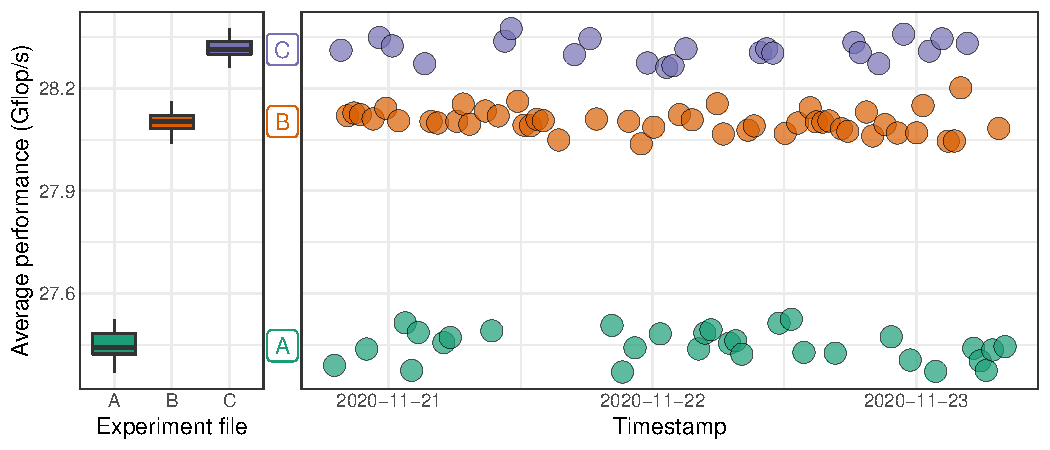
\includegraphics[width=\linewidth]{img/experiment/randomizing_sizes/expfile/average_performance.pdf}
                \caption{Average performance observed on CPU 1 of dahu-5, each point represents one experiment. A
                significant part of the variability is due to the choice of the experiment file.}%
                \label{fig:randomizing_sizes:expfile:average_perf}
            \end{figure}

            The effective performance is not the only aggregated metric affected by the choice of the experiment file.
            The distributions of two regression coefficients are represented in
            Figure~\ref{fig:randomizing_sizes:expfile:average_distribution}, namely the coefficients corresponding to
            the products \(MNK\) and \(NK\) (the effect of the experiment file on the coefficients for \(MK\) and \(MN\)
            is extremly similar to \(NK\)). It appears here that the experiment file causing the highest performance
            gives the highest cubic coefficient and the lowest quadratic coefficients. In other words, this means that
            with this experiment file, a larger fraction of the \dgemm durations is explained by the cubic coefficient.

            \begin{figure}[htpb]
                \centering
                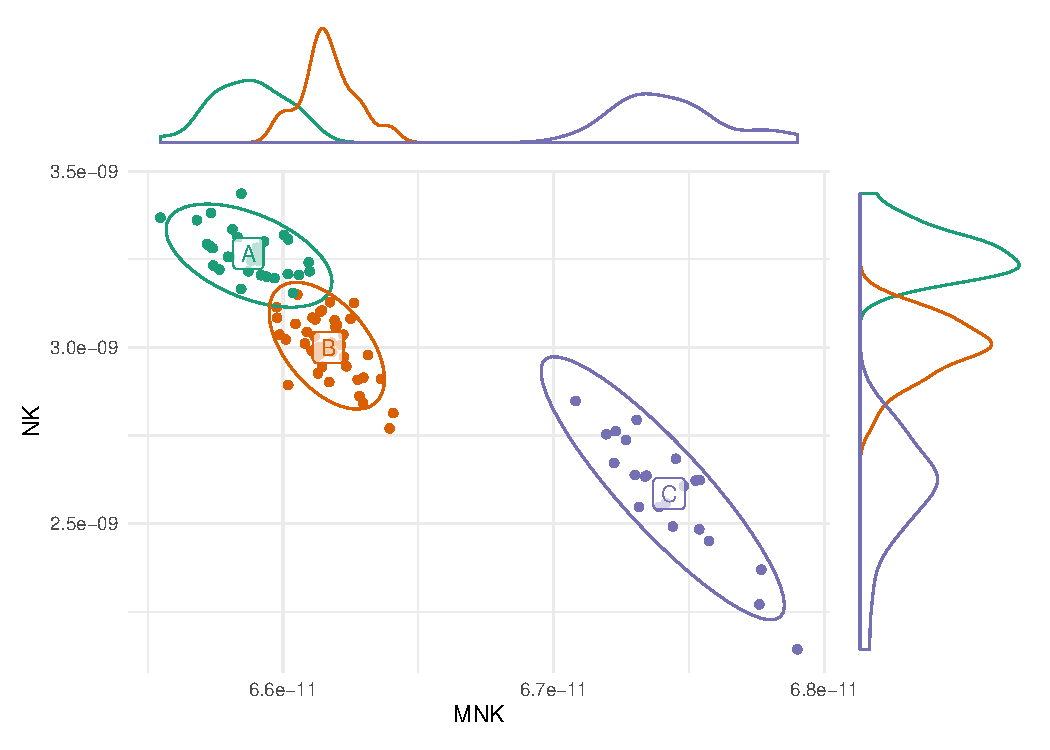
\includegraphics[width=\linewidth]{img/experiment/randomizing_sizes/expfile/average_distribution.pdf}
                \caption{Distribution of two of the regression parameters for CPU 1 of dahu-5, each point represents one
                experiment. The experiment file has a clear effect on the generated model}%
                \label{fig:randomizing_sizes:expfile:average_distribution}
            \end{figure}

            These observations suggest that experiments \texttt{A} and \texttt{B} may be less cache-friendly than
            experiment \texttt{C}, since in a matrix product the number of arithmetic operations grows cubically with
            the size of the input whereas the number of memory accesses grows quadratically.

            A non-aggregated view of the data is presented in Figure~\ref{fig:randomizing_sizes:expfile:raw_data}, each
            point represents one individual call to \dgemm. It appears that most of the calls in the three experiments
            have extremly similar durations for a given product \(MNK\). However, a small fraction of the \dgemm calls
            were significantly slower than the others with experiments \texttt{A} and \texttt{B}. All these calls have
            been made with a tall and skinny matrix, with \(K\geq3000\), which corroborates the hypothesis of a bad
            cache utilization.

            \begin{figure}[htpb]
                \centering
                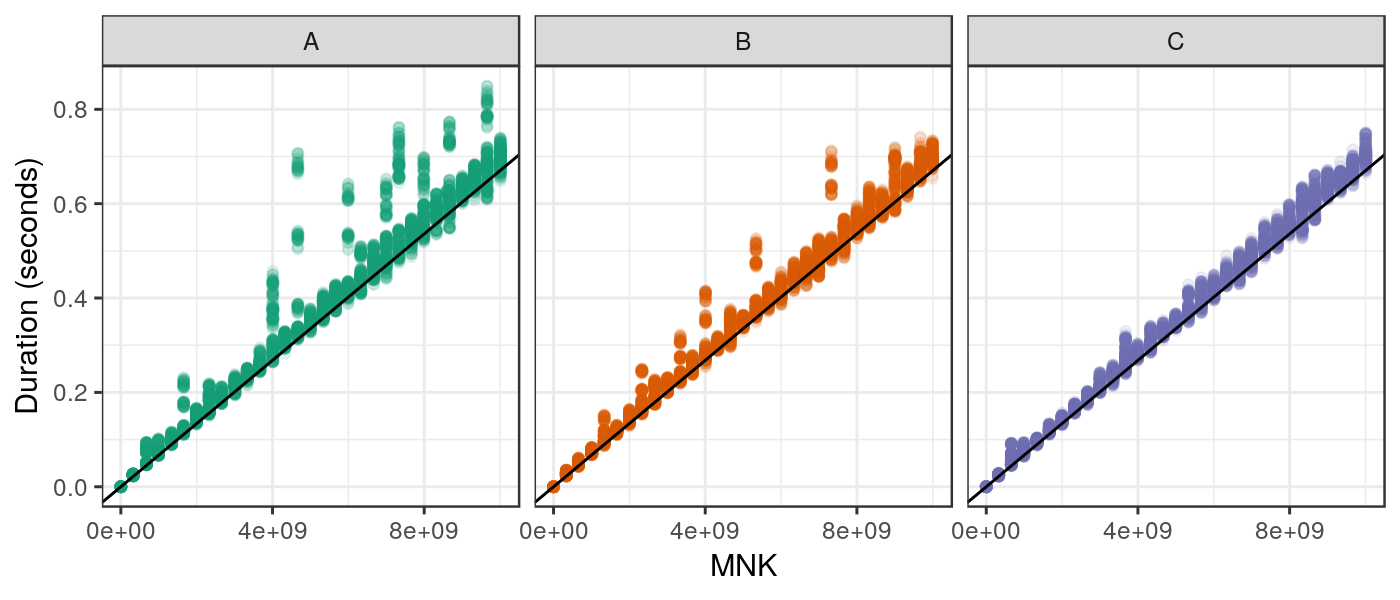
\includegraphics[width=\linewidth]{img/experiment/randomizing_sizes/expfile/raw_data.png}
                \caption{Durations of individual \dgemm calls for CPU 1 of dahu-5.
                Several calls have significantly longer durations than others. Identical black line on the three plots,
                with slope \Num{6.7e-11}.}%
                \label{fig:randomizing_sizes:expfile:raw_data}
            \end{figure}

            A final argument towards this hypothesis is presented with
            Figure~\ref{fig:randomizing_sizes:expfile:average_power}, the average DRAM power consumption during each run
            is presented. Similarly to Figure~\ref{fig:randomizing_sizes:expfile:average_perf}, there is a clear
            difference between the three experiments that cannot be explained by any temporal perturbation. Experiment
            \texttt{C}, which was the fastest, has the smallest DRAM power consumption. This suggests that the memory
            was used less intensively with this experiment, \ie there was a better cache utilization.

            \begin{figure}[htpb]
                \centering
                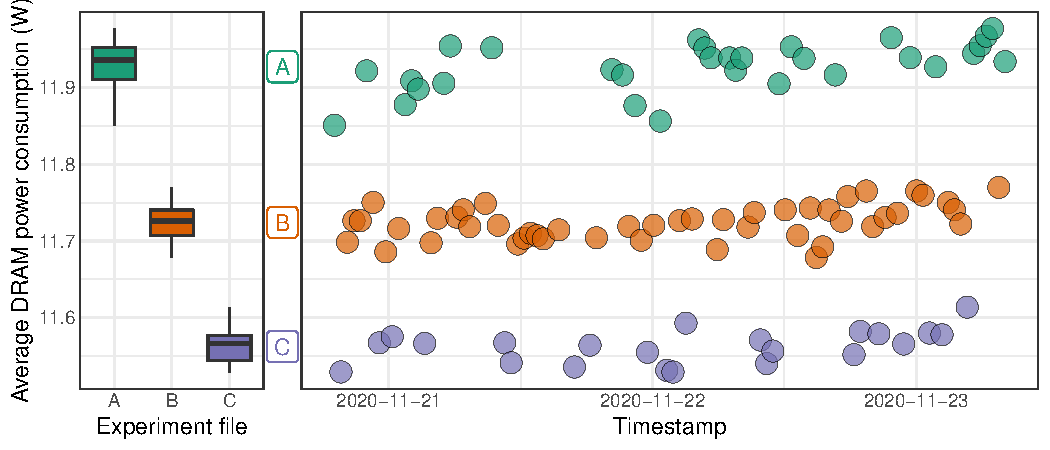
\includegraphics[width=\linewidth]{img/experiment/randomizing_sizes/expfile/average_power.pdf}
                \caption{Average DRAM power consumption observed on CPU 1 of dahu-5, each point represents one
                experiment.}%
                \label{fig:randomizing_sizes:expfile:average_power}
            \end{figure}

            In this section, we compared several \dgemm experiments performed with three sets of sizes. These sets have
            been generated according to the same statistical distribution, yet they lead to significantly different
            \dgemm models. We would like to stress that this discrepancy of the resulting models is due to a difference
            in the experimental conditions and not (only) to a statistical artifact. We proposed the hypothesis of a
            poor cache utilization, but other possibilities should not be dismissed, since this study was only
            observationnal, our hypothesis would need to be confirmed or refuted with a properly designed experimental
            study.

        \subsection{Effect of the experiment file generation method}%
        \label{sub:effect_experiment_file_generation_method}

            Section~\ref{sub:effect_experiment_file} has shown that the experiment file had a significant impact on the
            experimental conditions which affected the resulting statistical model. We generated three different
            sequence of sizes using the \emph{uniform product} method and performed several runs with each of these
            sequences.

            Now, we investigate briefly the effect of the generation method itself. We compare the \emph{independent
            sizes} and the \emph{uniform product} methods described in Section~\ref{sec:parameter_space}. For each of
            these methods, we generated several experiment files and performed one run with each of these files.

            Although there is a large variability, which is due to the use of several experiment files, it appears that
            the two generation methods lead to significantly different experimental conditions, as shown by
            Figure~\ref{fig:randomizing_sizes:expfile:method}. With the \emph{uniform product} method, \dgemm average
            performance is higher and the DRAM power consumption is lower.

            \begin{figure}[htpb]
                \centering
                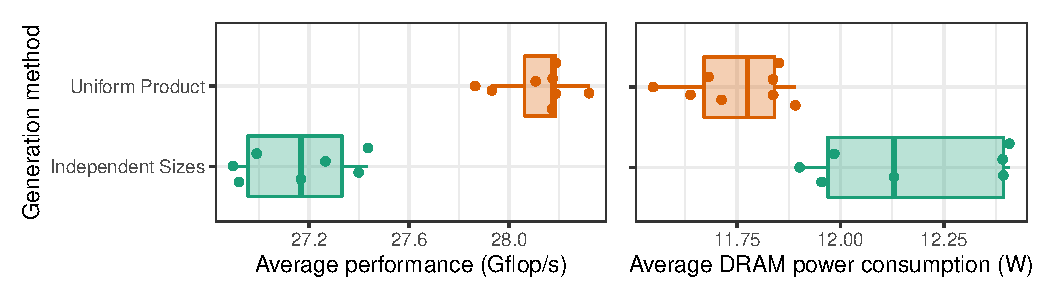
\includegraphics[width=\linewidth]{img/experiment/randomizing_sizes/method/average.pdf}
                \caption{Average \dgemm performance and power consumption observed on CPU 1 of dahu-5, each point
                represents one experiment.}%
                \label{fig:randomizing_sizes:expfile:method}
            \end{figure}


        \subsection{Effect of calibrating with a fixed size}%
        \label{sub:fixed_size}

            In the experiments described in Section~\ref{sub:effect_experiment_file} and
            Section~\ref{sub:effect_experiment_file_generation_method}, the three \dgemm parameters \(M\), \(N\) and
            \(K\) can take arbitrary values, to avoid any bias. One of the main reasons we make such measures is to
            generate a statistical model of \dgemm durations for simulating HPL. For this model to be faithful, the
            experimental conditions of our measures must be as realistic as possible to what happens during HPL
            execution. However, nearly all the \dgemm calls performed in HPL use the same value for the parameter \(K\),
            equal to HPL block size (\ie the parameter \texttt{NB}). For this reason, biasing the calibrations by using
            a fixed value for \(K\) could help to improve the simulation accuracy. This section investigates the
            question. We have generated five sets of experiment files:
            \begin{description}
                \item[Random] This is the usual \emph{uniform product} generation procedure already discussed in
                    previous sections.
                \item[Fixed K] We modified the \emph{uniform product} procedure to have a constant value for \(K\). We
                    generated three sets of files, with \(K=128\), \(K=256\) and \(K=512\).
                \item[Several fixed K] We modified the \emph{uniform product} procedure to have the value of \(K\)
                    choosen randomly in \{128,256,512\}. This is equivalent to concatenating three files generated with
                    the \emph{fixed K} method and then shuffling the resulting file.
            \end{description}
            For each of the five experiment kinds, we have generated several dozen of experiment files. Then, we
            performed one experiment with each of these files in a random order during a week-end on two nodes of the
            dahu cluster for a total of four different processors. Again the results are similar for all of them, so we
            will focus on a single processor.

            Figure~\ref{fig:randomizing_sizes:expfile:fixing_K:performance} presents the observed \dgemm performance
            with the five experiments. We can observe that again, the generation method for the size sequence has a huge
            effect on the experiment. First, using a fixed value for \(K\) reduces very significantly the inter-run
            performance variability. The average performance is also greatly affected, it is the highest with \(K\)
            fixed to 128, the lowest with \(K\) fixed to 256 or 512 or with the random generation, and it is
            intermediate with \(K\) randomly sampled in \(\{128,256,512\}\).

            \begin{figure}[htpb]
                \centering
                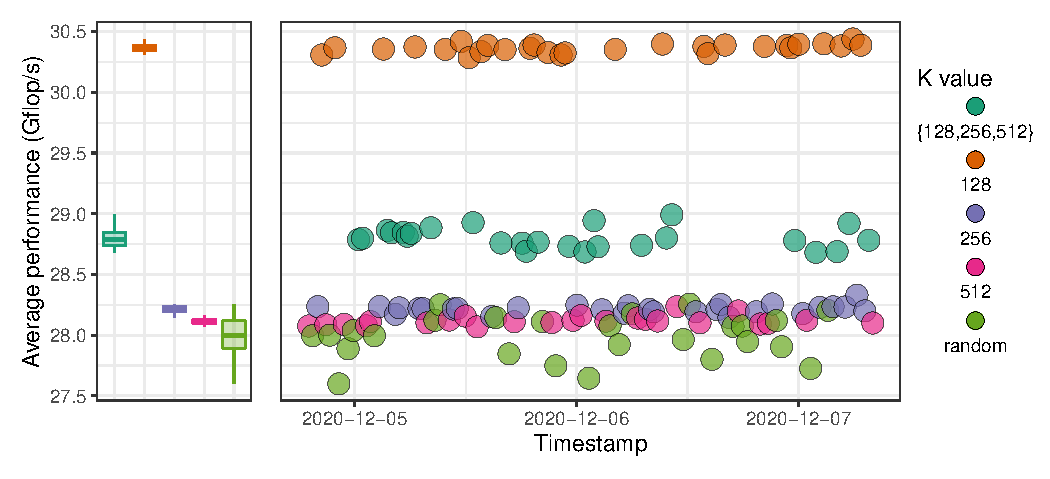
\includegraphics[width=1\linewidth]{img/experiment/randomizing_sizes/fixing_K/average_performance.pdf}
                \caption{Average \dgemm performance observed on CPU 1 of dahu-5, each point represents one experiment.}%
                \label{fig:randomizing_sizes:expfile:fixing_K:performance}
            \end{figure}

            The monitoring data collected during the experiments also reveal interesting differences. The average CPU
            frequency is reported in Figure~\ref{fig:randomizing_sizes:expfile:fixing_K:frequency}. It appears that the
            frequency is the highest with \(K=128\) and with the random experiment. It is significantly lower with \(K\)
            chosen randomly among the three sizes, and even lower with \(K=256\) and \(K=512\). It is interesting to
            note that there is a positive correlation between the frequency and \dgemm performance, but the random
            experiment is a clear exception as it leads to a relatively low performance and high frequency.

            \begin{figure}[htpb]
                \centering
                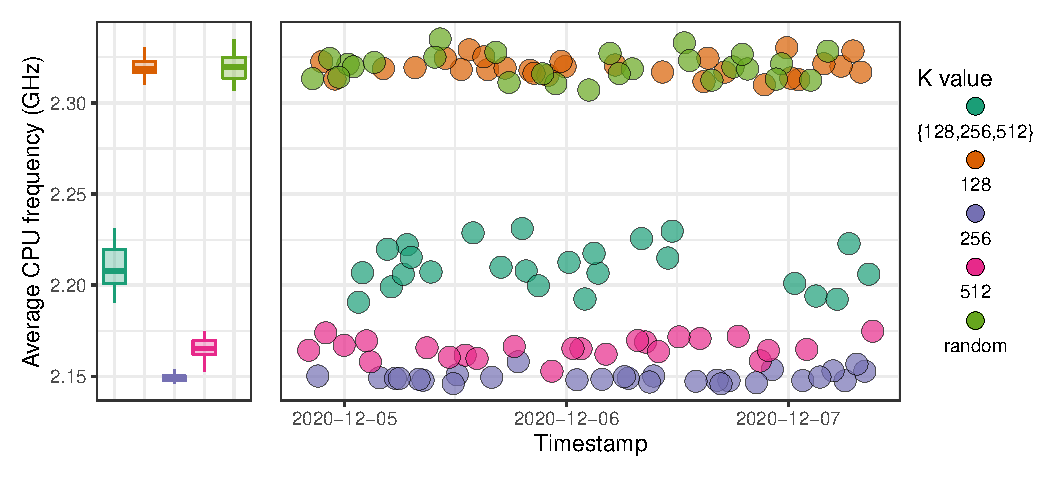
\includegraphics[width=1\linewidth]{img/experiment/randomizing_sizes/fixing_K/average_frequency.pdf}
                \caption{Average CPU frequency, observed on CPU 1 of dahu-5, each point represents one experiment.}%
                \label{fig:randomizing_sizes:expfile:fixing_K:frequency}
            \end{figure}

            The average CPU power consumption, presented in
            Figure~\ref{fig:randomizing_sizes:expfile:fixing_K:power_CPU}, is particularly peculiar. The random
            experiment has a power consumption significantly lower and more variable than the four other experiments
            that are all extremly stable, with nearly no inter-run variability. This observation is very
            counter-intuitive, since the CPU power consumption is in general proportional to the CPU
            frequency~\cite{heinrich:hal-01523608}.  This only happens on the CPU 1 of the two nodes we tested, the
            power consumption of the CPU 0 is extremly stable and similar for the five experiment kinds.

            \begin{figure}[htpb]
                \centering
                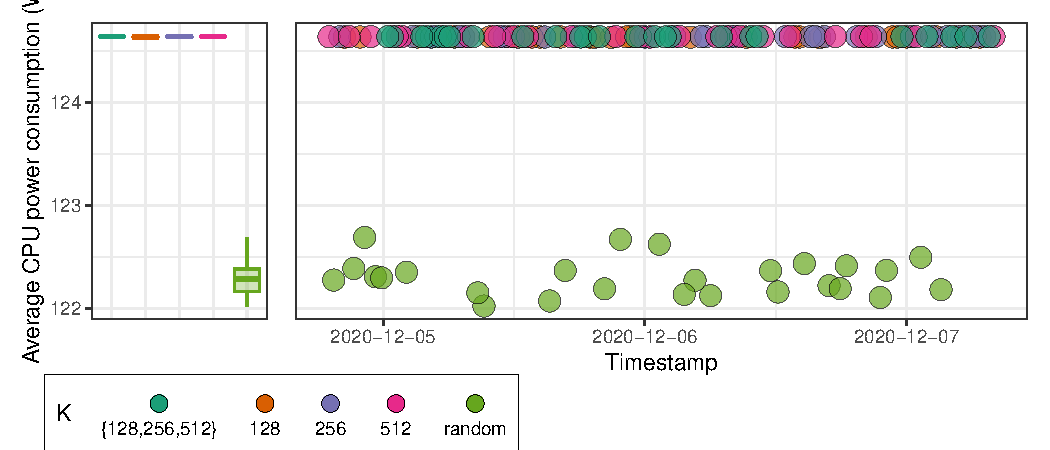
\includegraphics[width=1\linewidth]{img/experiment/randomizing_sizes/fixing_K/average_power_CPU.pdf}
                \caption{Average CPU power consumption, observed on CPU 1 of dahu-5, each point represents one experiment.}%
                \label{fig:randomizing_sizes:expfile:fixing_K:power_CPU}
            \end{figure}

            The five experiments exhibit very different average DRAM power consumption, as depicted in
            Figure~\ref{fig:randomizing_sizes:expfile:fixing_K:power_DRAM}. The experiment with \(K=128\) is the most
            energy-hungry, followed by the experiment with \(K\in\{128,256,512\}\), then the experiments with a random
            \(K\), \(K=256\) and \(K=512\). It is interesting to note that the experiment with the highest DRAM power
            consumption is also the one with the highest average \dgemm performance, which is the opposite of what was
            observed in Section~\ref{sub:effect_experiment_file}.
            \begin{figure}[htpb]
                \centering
                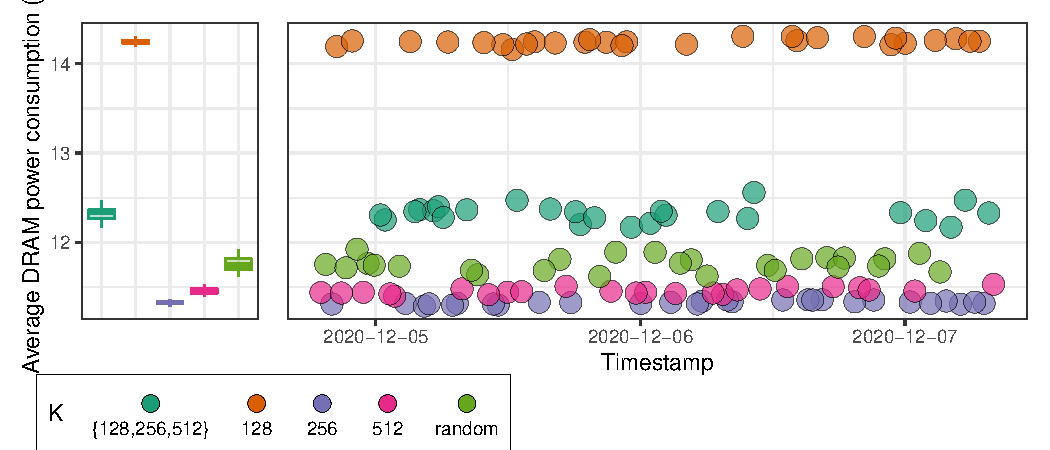
\includegraphics[width=1\linewidth]{img/experiment/randomizing_sizes/fixing_K/average_power_DRAM.pdf}
                \caption{Average DRAM power consumption, observed on CPU 1 of dahu-5, each point represents one experiment.}%
                \label{fig:randomizing_sizes:expfile:fixing_K:power_DRAM}
            \end{figure}

            Finally, the performance of individual \dgemm calls are presented in
            Figure~\ref{fig:randomizing_sizes:expfile:fixing_K:raw_data}. We made the observation earlier that there was
            much less inter-run variability when the value of \(K\) was fixed. This plot shows that there is also
            significantly less intra-run variability. Furthermore, we can compare the performance of \dgemm for a given
            value of \(K\). With \(K=128\), the performance is higher in the experiment where all the calls are done
            with \(K=128\) than in the experiment with \(K\in\{128,256,512\}\). With the two other values, \(K=256\) and
            \(K=512\), this is the opposite, the performance is higher in the mixed experiment than in the experiment
            with only one \(K\) value. This shows that the durations of individual \dgemm calls are not independent, one
            call can be faster or slower depending on the calls previously made.
            \begin{figure}[htpb]
                \centering
                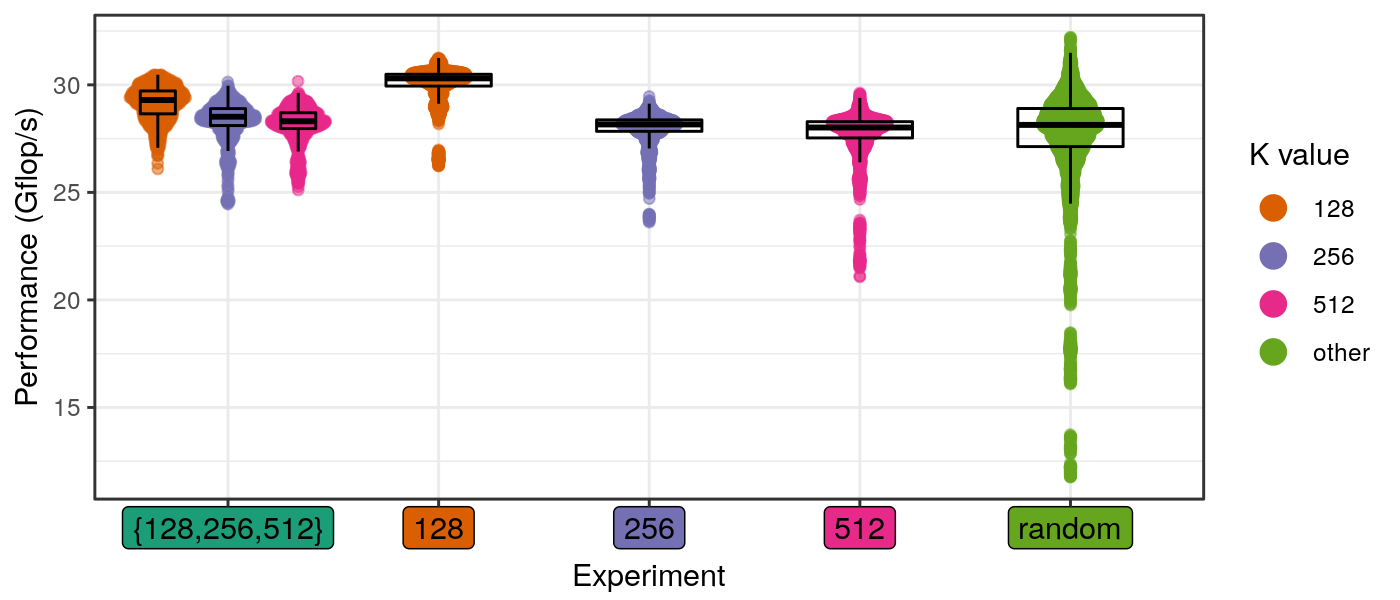
\includegraphics[width=1\linewidth]{img/experiment/randomizing_sizes/fixing_K/raw_data.png}
                \caption{Durations of individual \dgemm calls for CPU 1 of dahu-5.}%
                \label{fig:randomizing_sizes:expfile:fixing_K:raw_data}
            \end{figure}

            In this section, we demonstrated once again that the sampling method has an important effect on the measured
            performance. This will affect any statistical model we could build using the measured data, not because of a
            statistical bias, but because of an experimental bias. Such a bias might be desirable, for instance it
            should help improve the prediction accuracy of our HPL simulations. It comes at a price though, since we
            need to perform a new \dgemm calibration if we want to simulate HPL with another block size.

    \section{Randomizing the data}%
    \label{sec:randomizing_data}
        %% TODO
        %% - Les performances de dgemm dépendent du contenu de la matrice (random ou
        %%   constant par exemple). Ça serait causé par des bit flips dans le CPU qui
        %%   engendre une plus grande consommation (réutiliser le rapport).
        The work presented in this section has been published as a technical report\cite{cornebize:bitflips}. The
        content of this section is therefore a near-verbatim copy of this report.

        This experiment comes, yet again, from an unfortunate phenomenon we stumbled upon when calibrating the platform
        for our simulations. Our predictions were wrong, so we investigated a bit and we noticed a significant mismatch
        between the durations measured with our calibration code and the durations observed in HPL. We found out that,
        the performance of the \dgemm function depends on the content of the matrix, which was unexpected.

        \subsection{Randomization of the matrix initialization}
        \label{sub:randomization_matrix_initialization}
            The three matrices are allocated once at the start of the program as a buffer of size \(N^2\) with
            \(N=2,048\). Then, their content is initialized in three different ways, depending on the experiment:
            \begin{enumerate}
                \item All the elements of the matrices are equal to some constant. We have tested with three different
                    values: 0, 0.987 and 1.
                \item The elements of the matrices are made of an increasing sequence in the interval \([0, 1]\). More
                    precisely, \texttt{mat[i] = i/(N\textasciicircum{}2-1)} for i in \([0, N^2-1]\).
                \item Each element of the matrix is randomly and uniformly sampled in the interval \([0, 1]\).
            \end{enumerate}

        Figure~\ref{fig:exp:bit-flips:method-perf} shows the evolution of the dgemm durations during the experiment.
        A clear temporal patterns can be distinguished, the performance is oscillating.  Furthermore, several layers can
        be seen, the durations of \dgemm are the highest when the matrices are initialized randomly and the
        lowest when they are initialized with a constant value. The sequential initialization is in between.

        \begin{figure}[htbp]
            \centering
            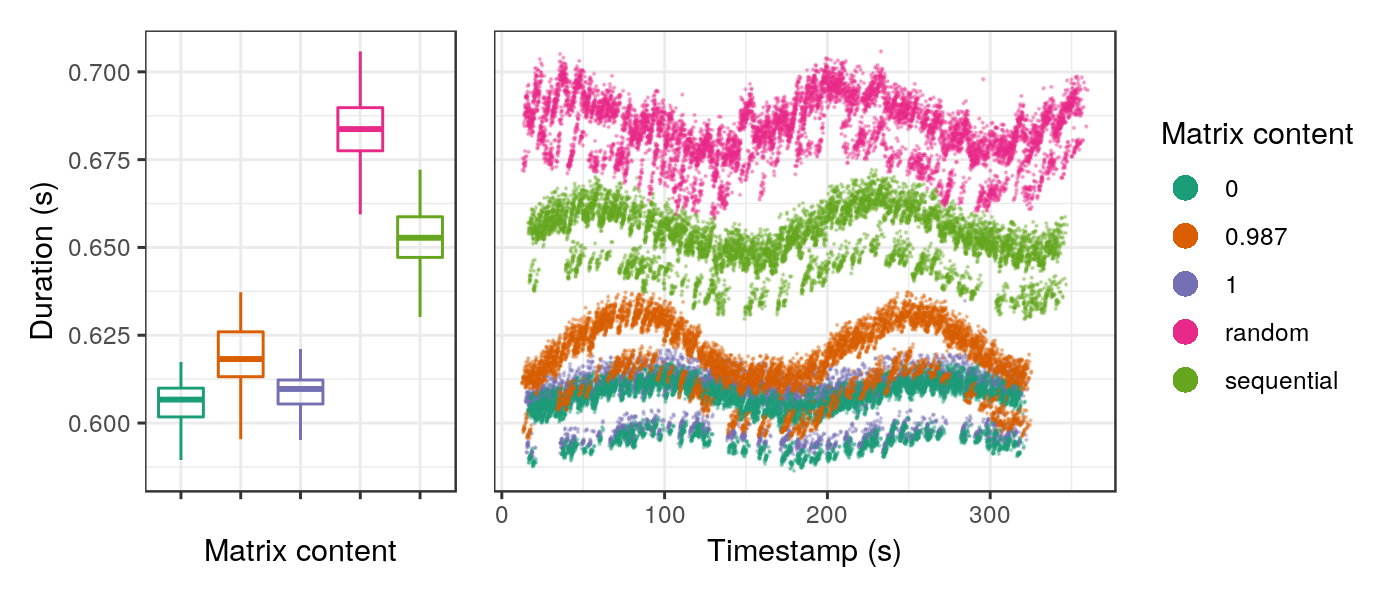
\includegraphics[width=\linewidth]{img/experiment/bit-flips/generation_method_perf.png}
            \caption{\label{fig:exp:bit-flips:method-perf}
            DGEMM durations are lower with constant values in the matrices}
        \end{figure}

        Such an observation was unforeseen. The function \dgemm implements the usual matrix product with cubic
        complexity. The control flow of the function does not depend on the matrix content, so we did not expect its
        duration to be data-dependent.

        The observations we have made on \dgemm performance can be explained by
        Figure~\ref{fig:exp:bit-flips:method-freq} which shows the evolution and the distribution of the core
        frequencies during the experiment. There is a clear correlation between the frequencies and \dgemm
        performance: the random initialization produces lower frequencies whereas the constant initialization gives
        higher frequencies. A similar temporal patterns can also be distinguished with clear oscillations.

        \begin{figure}[htbp]
            \centering
            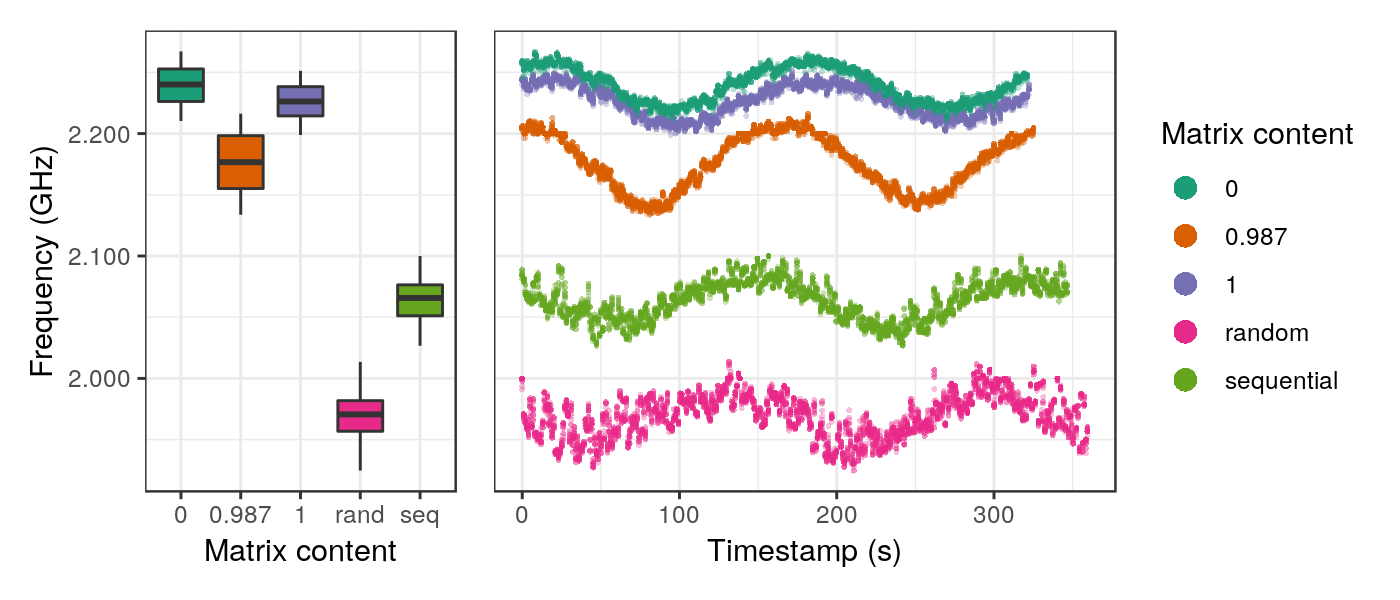
\includegraphics[width=\linewidth]{img/experiment/bit-flips/generation_method_freq.png}
            \caption{\label{fig:exp:bit-flips:method-freq}
            Core frequencies are higher with constant values in the matrices}
        \end{figure}

        This experiment has been repeated on other Grid'5000 clusters, each time on at least four distinct nodes.
        Table~\ref{tab:bit-flips} gives a summary of our observations. Five other clusters show a similar behavior, the
        performance of \dgemm is higher when the matrices are generated with a constant value. However, for five
        other clusters, this phenomenon could not be observed, the matrix content had no impact on the performance.
        %% TODO run this experiment on other Grid'5000 clusters, just to extend a bit the table of the clusters we tested it on.
        %% I have at least two clusters in mind:
        %% - pyxis (ARM processors)
        %% - troll (newest generation of Intel processors, Cascade Lake)

        \begin{table}[htbp]
            \caption{\label{tab:bit-flips}
            Observation of the  performance anomaly on Grid'5000 clusters}
            \centering
            \begin{tabular}{lllll}
                \toprule
                Cluster & CPU & Generation & Release date & Anomaly\\
                \midrule
                nova & Intel Xeon E5-2620 v4 & Broadwell & Q1'12 & no\\
                taurus & Intel Xeon E5-2630 & Sandy Bridge & Q1'12 & no\\
                ecotype & Intel Xeon E5-2630L v4 & Broadwell & Q1'12 &yes\\
                paranoia & Intel Xeon E5-2660 v2 & Ivy Bridge & Q3'13 & no\\
                parasilo & Intel Xeon E5-2630 v3 & Haswell & Q3'14 & yes\\
                chiclet & AMD EPYC 7301 & - & Q2'17 & no\\
                dahu & Intel Xeon Gold 6130 & Skylake & Q3'17 & yes\\
                yeti & Intel Xeon Gold 6130 & Skylake & Q3'17 &yes\\
                pyxis & ARM ThunderX2 99xx & - & Q2'18 & no\\
                gros & Intel Xeon Gold 5220 & Cascade Lake & Q2'19 & yes\\
                troll & Intel Xeon Gold 5218 & Cascade Lake & Q2'19 & yes\\
                \bottomrule
            \end{tabular}
        \end{table}

        \subsection{Hypotheses}
            %% TODO add the hypothesis on subnormal numbers.
            Several hypotheses were discussed to explain this unexpected phenomenon.

            There could be a small cache  on the floating point unit of the cores to memorize the results of frequent
            operations. This could explain why the durations were higher when the matrices were initialized randomly,
            but this does not explain why the sequential initialization is in between.

            This could be due to kernel same page merging (KSM), a mechanism that allows the kernel to share identical
            memory pages between different processes. Again, this would explain the difference between the random
            initialization and the constant one, but not why the sequential initialization gives intermediate
            performance.

            A last hypothesis is the power consumption of the cores. Each state change of the electronic gates of the
            CPU costs an energy overhead. In the case of the constant initialization, the registers will change less
            often during the execution of \dgemm, in comparison with the random initialization. Thus, with the
            constant initialization, the processor cores would be able to maintain a higher frequency while respecting
            the thermal design power (TDP), with the random initialization the frequency would be throttled more
            aggressively and thus the performance would be lower.
            As for the sequential initialization, we can imagine that we have a locality effect: nearby elements of the
            matrices will have more bits in common, this would causes less bit flips than the random initialization but
            more bit flips than the constant initialization and thus an intermediate performance.

        \subsection{Testing the bit-flip hypothesis}
            To test the hypothesis that the lower frequencies are caused by more frequent bit flips in the processor,
            the matrix initialization has been changed. Now, each element of the matrix is randomly and uniformly
            sampled in the interval \([0,1]\). Then a bit mask is applied on the lower order bits of their mantissa. As
            a result, all the elements of the matrices have some bits in common. This method is illustrated in
            Figure~\ref{fig:exp:bit-flips:mask_illustration}, the mantissa of the matrix elements (in blue) is at first
            completely random, then we apply a mask so that the right-most bits (in green) become
            deterministic\footnote{Image adapted from
            \url{https://en.wikipedia.org/wiki/Double-precision_floating-point_format}}.  Several mask sizes have been
            tested, from 0 (the elements are left unchanged) to 53 (the mantissa becomes completely deterministic, all
            the elements are equal).
            \begin{figure}[htpb]
                \begin{center}
                    \includesvg[width=\linewidth]{img/experiment/bit-flips/float.svg}
                    \vspace{-0.2cm}

                    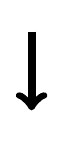
\begin{tikzpicture}
                        \draw[->, line width=1mm] (0,0) -- (0,-1);
                    \end{tikzpicture}

                    \vspace{-0.2cm}
                    \includesvg[width=\linewidth]{img/experiment/bit-flips/float_mask.svg}
                \end{center}
                \caption{Illustrating the effect of applying a mask on the random part of the matrix
                elements\label{fig:exp:bit-flips:mask_illustration}}
            \end{figure}

            The evolution and the distribution of the \dgemm durations is plotted in
            Figure~\ref{fig:exp:bit-flips:mask-perf}. Their is a very clear correlation between the mask size and the
            performance: the larger the mask, the lower the duration. Similarly to the previous experiment, some
            temporal patterns can also be distinguished.

            \begin{figure}[htbp]
                \centering
                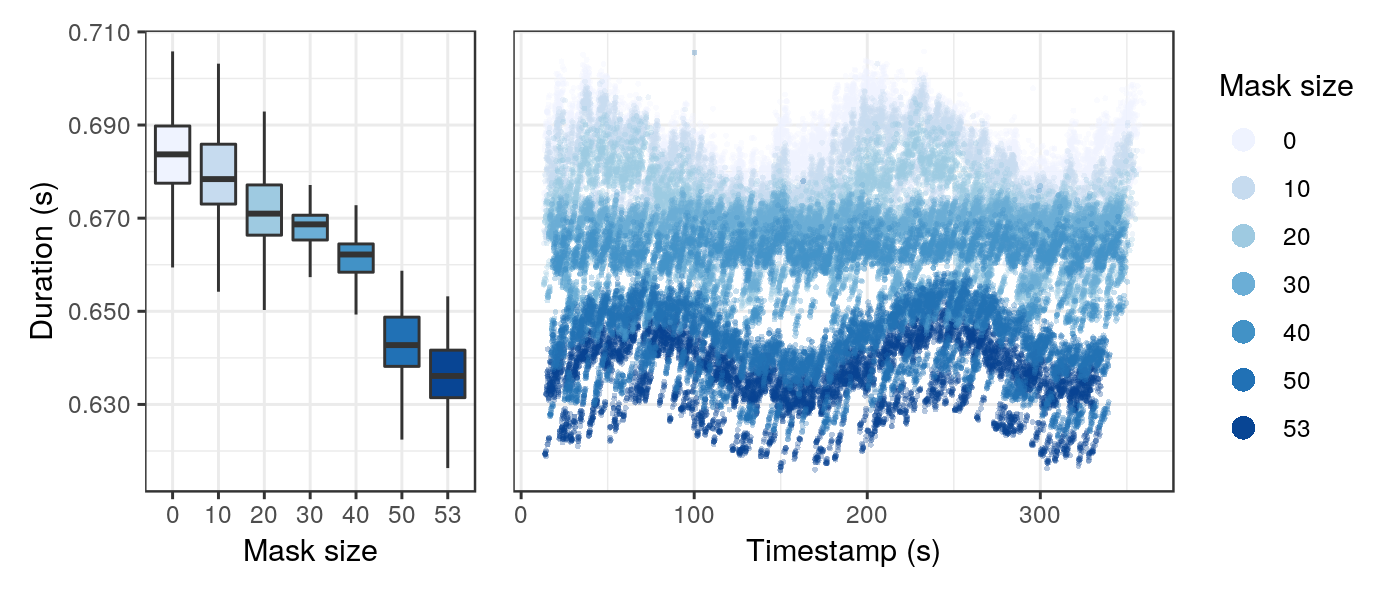
\includegraphics[width=\linewidth]{img/experiment/bit-flips/mask_size_perf.png}
                \caption{\label{fig:exp:bit-flips:mask-perf}
                DGEMM durations are lower with larger bit masks}
            \end{figure}

            This correlation with the mask size can also be seen with the frequencies in
            Figure~\ref{fig:exp:bit-flips:mask-freq}: larger masks lead to higher frequencies.

            \begin{figure}[htbp]
                \centering
                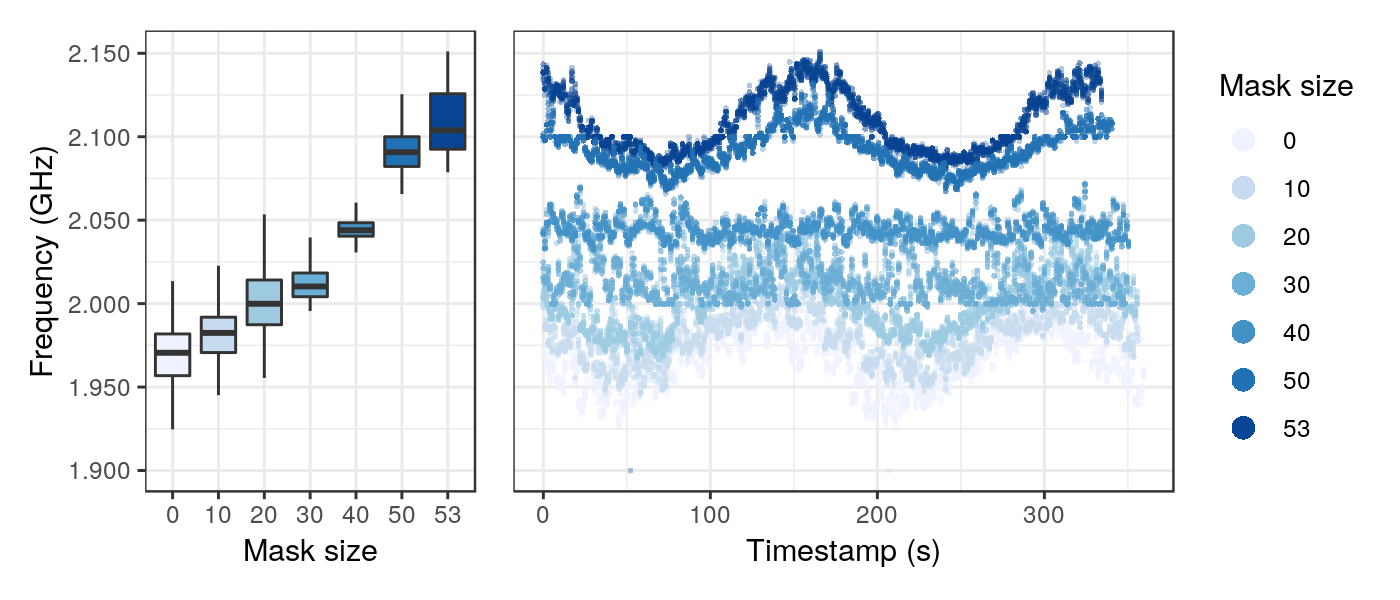
\includegraphics[width=\linewidth]{img/experiment/bit-flips/mask_size_freq.png}
                \caption{\label{fig:exp:bit-flips:mask-freq}
                Core frequencies are higher with larger bit masks}
            \end{figure}

            This experiment has been repeated on two other Grid'5000 clusters, ecotype and gros. For both of them, the
            same observations could be made, a clear correlation between the mask size, the frequencies and the
            performance.

        \subsection{Conclusion}
            We have shown that the performance of the \dgemm function is data-dependent. The best explanation we
            have for this counter-intuitive fact is an energy cost overhead caused by bit flips inside the processor.
            To respect its energy budget, the CPU has to throttle more aggressively its frequency when the matrices
            content is more diverse and thus more energy consumming.
            This theory has been corroborated by a controlled experiment where the elements of the matrices are
            initialized semi-randomly: they all share an identical bit suffix.

            To strengthen this claim further, the next steps will be to perform a similar experiment with another
            compiler, another BLAS library and/or another computation kernel. We also need to understand why some
            processors are subject to this phenomenon and some others are not.

            We warmly thank our colleagues that helped us to find hypotheses for this performance anomaly. In
            particular, Guillaume Huard suggested that the performance anomaly may be caused by the bit flips in the
            processor.

        \subsection{Related work}%
            M. La{\ss}, C. Plessl and R. Schade (Paderborn Center for Parallel Computing) made independently similar
            observations (personal communications on 2020/09/24 and 2020/11/11). Their findings is summarized here:
            \begin{itemize}
                \item They observed that \dgemm performance depended on the content of the matrix. They also
                    made the hypothesis that it was caused by bit-flips. To test this hypothesis, they used the same
                    approach, they filled the matrices with random values with a mask applied to the lower-order bits.
                    They observed a correlation between the mask size and \dgemm performance, which is an
                    argument in favor of this hypothesis. This experiment was done using anoter \dgemm
                    implementation than us (Intel MKL) on an Intel Xeon Gold 6148 (Skylake-SP family) from a noctua
                    node\footnote{\url{https://pc2.uni-paderborn.de/hpc-services/available-systems/noctua/}}.
                \item They reproduced the same experiment on a FPGA (more precisely, a Bittware 520N PCIe accelerator
                    card, equipped with an Intel Stratix 10 GX 2800 FPGA). This time, the way the matrix was filled had
                    an effect on the power consumption and not the performance. This was expected since there is no DVFS
                    on FPGA.
                \item To see whether the effect was caused by the CPU arithmetic units or the cache, they adapted a
                    micro-benchmark\footnote{\url{https://github.com/pc2/Flops}} to perform multiplications with more or
                    less random data, using only the registers of the CPU. They did not observe any difference of
                    performance caused by the data, but they did observe a higher power consumption of \SI{5}{\percent}
                    with random data. This power consumption remained under the TDP even after the increase, so the CPU
                    frequency did not get throttled.
            \end{itemize}

            Sch{\"{o}}ne~\etal~\cite{DBLP:journals/corr/abs-1905-12468} observed a data-dependent power consumption with
            a Skylake-SP processor using AVX instructions. Note that in their experiment, the core frequency and the
            instruction rate were constant.

            Andr\'e~\etal~\cite{andre:hal-02401796} observed in one of their experiments that limiting the uncore
            frequency (\ie the frequency of the L3 cache and the memory controler) can increase the performance of HPL
            by about \SI{1.5}{\percent}. The reason is that HPL power consumption reaches TDP, so lowering the uncore
            frequency allows a higher power consumption of the cores and thus a higher frequency.

    \section{Beware of extrapolations}%
    \label{sec:beware_of_extrapolations}
        %% TODO
        %% Le problème est survenu dans plusieurs cas de figure, notamment
        %% pour HPL avec des géométries très élongées.
        %% - Les prédictions pour dgemm n'étaient plus très bonnes. On extrapolait trop
        %%   loin, la calibration était faite avec M<=15000 et N<=15000 alors que pour de
        %%   telles géométries on avait parfois des tailles 10\times plus grandes (les
        %%   produits MNK avaient le même ordre de grandeur par contre).
        %% - Les prédictions pour les communications étaient également mauvaises, en
        %%   partie parce que l'on calibrait pour des messages jusqu'à 1MB et on
        %%   esssayait de prédire la durée de communications de 1GB.
        Some text\dots

    \section{Beware of experimental conditions}%
    \label{sec:beware_of_experimental_conditions}
        %% TODO
		%% - Chauffe des CPU avant au cas où. Brice et Kevin monitoraient la
		%%   température au fil de l'expérience et arrêtaient les mesures quand
		%%   c'était trop chaud.
		%% - Dans HPL, il semble que les calculs ralentissent beaucoup certaines
		%%   communications. Ce phénomène n'était initialement pas capturé par la
		%%   calibration puisque les mesures étaient faites sans aucun calculs à
		%%   côté.
        Some text\dots

	\section{Conclusion}
		%% TODO
        %% - Certains facteurs extérieurs peuvent grandement impacter l'expérience, exemple
        %%   des problèmes de température sur dahu-{13,14,15,16}. D'où la nécessité de (1)
        %%   contrôler d'avantage l'environnement et (2) collecter d'avantage
        %%   d'informations sur l'environnement.
        Some text\dots


\chapter{Performance non-regression tests}%
\label{chapter:experiment:tests}
    %% TODO
    %% La partie précédente a montré que de nombreux problèmes peuvent survenir sur un
    %% testbed comme Grid'5000. Certains sont très visibles et vont être détectés
    %% rapidement (e.g. un disque HS), d'autres sont plus subtiles et peuvent passer
    %% inaperçu, faussant donc les expériences (e.g. performance inférieure de quelques
    %% pourcents). Dans cette partie, on essaye de détecter ces problèmes
    %% automatiquement.

    \section{State of the art}%
        %% TODO comment font les GAFAM ?
        Some text\dots

    \section{Performance measure and information collection}%
    \label{sec:performance_measure_and_information_collection}
        %% TODO
        %% Description du workflow mis en place, avec un joli dessin.
        %% - Génération du fichier d'expérience.
        %% - Soumission de jobs sur chaque cluster.
        %% - Réalisation de l'expérience, entièrement gérée par peanut.
        %% - Push automatique des résultats sur le dépôt gitlab.
        %% - Soumission d'un job CI pour extraire et agréger les informations des archives.
        %% - Réalisation des tests et courbes sur les données.
        Some text\dots

    \section{Statistical test}%
    \label{sec:statistical_test}

        The following is a transcription of section 4.4 of Chew~\cite{chew}.\footnote{This publication, dating from
        1966, is the oldest paper used in this thesis. It has been written by an employee of RCA Service Co., a
        contractor of the US Air Force. The author of the paper describes the typical use case: computing the
        coordinates of a prediction ellipse for the splash point of a future missile shot.}
        \begin{quote}
            Suppose that we have already observed \(n\) vectors of dimension \(p\): \(\bm{x_1},\dots,\bm{x_n} \in
            \mathbb{R}^p\). We define the random variable \(\bm{m}^{(r)}\) to be the sample mean of the next (unknown)
            \(r\) observations: \(\bm{m}^{(r)}= \frac{\bm{x_{n+1}}+\dots+\bm{x_{n+r}}}{r}\). We assume here that all the
            \(\bm{x_i}\) are independent.

            Then, the prediction region of \(\bm{m}^{(r)}\) with probability \(\gamma\) is:
            \[
            \frac{nr}{n+r} (\bm{m}^{(r)} - \overline{\bm{x}})^T \bm{S}^{-1}(\bm{m}^{(r)} -
            \overline{\bm{x}})
            =
            \frac{(n-1)p}{n-p} Q_F(1-\gamma, p, n-p)
             \]
            Where \(\overline{\bm{x}}\) and \(\bm{S}\) are respectively the sample mean and sample covariance matrix of
            the \(n\) observed \(\bm{x_i}\), and \(Q_F(\alpha,v_1,v_2)\) denotes the upper \(\alpha\) quantile of
            \(F(v_1, v_2)\), the F-distribution with \(v_1\) and \(v_2\) degrees of freedom.
        \end{quote}

        A test could therefore be designed as follows:

        Compute the value \(t\):
        \[
        t = \frac{nr(n-p)}{(n+r)(n-1)p} (\bm{m}^{(r)} - \overline{\bm{x}})^T \bm{S}^{-1}(\bm{m}^{(r)} -
        \overline{\bm{x}})
         \]

        Then, raise an error if \(t \geq Q_F(0.95, p, n-p)\).  Note that there is no closed form for the value \(Q_F\),
        but it can be obtained (numerically) in R with the function
        \texttt{qf}\footnote{\url{https://stat.ethz.ch/R-manual/R-devel/library/stats/html/Fdist.html}} and in Python
        with the function
        \texttt{scipy.stats.f.ppf}\footnote{\url{https://docs.scipy.org/doc/scipy/reference/generated/scipy.stats.f.html}}.
        The \([0.05,0.95]\) interval should be adapted empirically.

        The proposed test is illustrated in Figure~\ref{fig:non_regression:stat:single_point}. A large number of points,
        in black, have been generated according to a known bivariate normal distribution. Their abscissa (resp.
        ordinate) are distributed according to a normal distribution of mean \(\mu_x\) and standard deviation
        \(\sigma_x\) (resp. \(\mu_y\) and \(\sigma_y\)). The abscissa and ordinates of the points are not independent,
        they have a correlation coefficient of -0.7. The \NSI{99.5}{\percent} prediction regions are shown in blue. Two
        additional points are shown in the scatter plot, representing new observations. The orange point has coordinates
        \((\mu_x+2\sigma_x,\mu_y+2\sigma_y)\) and the green point has coordinates \((\mu_x+2\sigma_x,\mu_y-2\sigma_y)\).

        If each dimensions were considered independently, we would conclude that the probabilities to observe the orange
        point or the green point are equal. Indeed, these two points have equivalent positions in the one-dimension
        density graphs and they both fall within the \NSI{99.5}{\percent} interval. Now, when we look at both dimensions
        simultaneously, the green point becomes much more likely to be observed, it is within the blue ellipse while the
        orange point is outside.

        \begin{figure}[htpb]
            \centering
            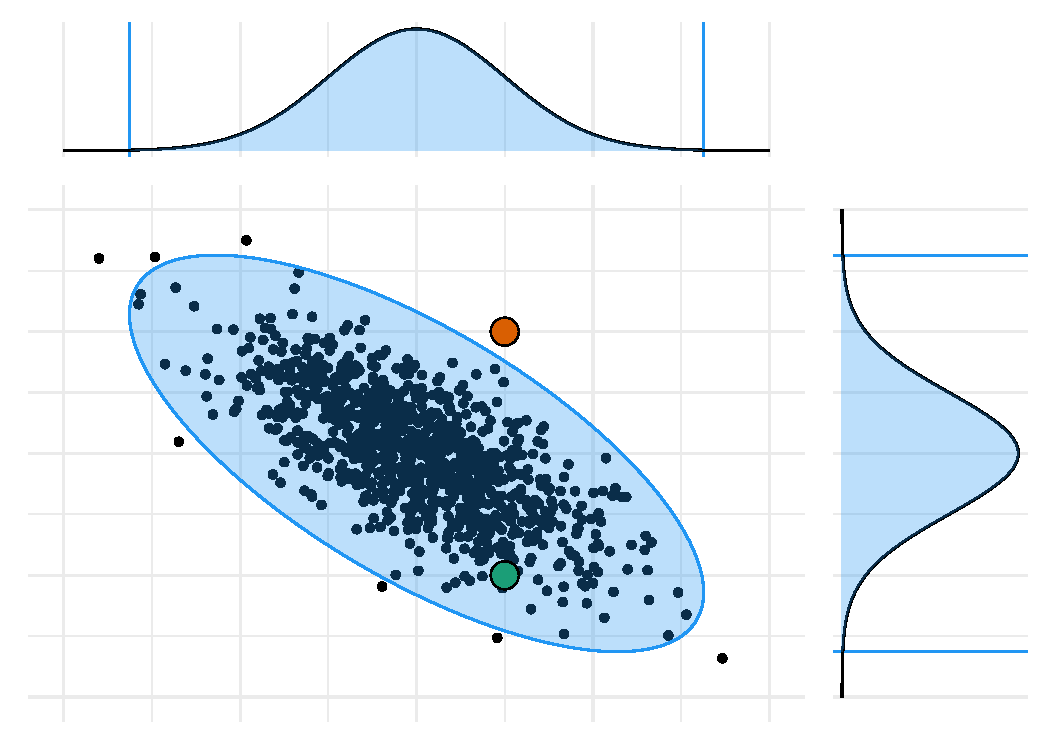
\includegraphics[width=1\linewidth]{img/experiment/non_regression/statistics/single_point.pdf}
            \caption{Illustrating the proposed test with two sets of one observation (\(r=1\)) and a bivariate normal
            distribution (\(p=2\)). The blue lines represent the \NSI{99.5}{\percent} prediction regions.}%
            \label{fig:non_regression:stat:single_point}
        \end{figure}

    \section{Conclusion}%
    \label{sec:conclusion}
        %% TODO
        %% Raconter ce que l'on aurait pu faire et comment il faudrait l'étendre:
        %% - Test sur le modèle de dgemme plutôt que sur l'aggregated gflops
        %% - Test du modèle MPI (si on arrivait à définir et calculer les IC)
